\chapter{Teoria di Lee - Yang e Modello di Ising}
Uno dei contributi più importanti in Meccanica statistica per comprendere le transizioni di fase proviene dalla teoria di Lee - Yang riguardante la struttura generale della funzione di partizione canonica. In particolare, i teoremi di Lee - Yang dimostrano come le transizioni di fase emergano solamente nel limite termodinamico. Per semplicità, ci si limita alla trattazione classica, ma con le medesime assunzioni anche la trattazione quantistica porterebbe agli stessi risultati. 

Si parte riconsiderando un potenziale di interazione della forma vista nella \eqref{eq: potenziale Lennard-Jones approx.} e in figura \ref{fig: potenziale coefficiente a2}, essenzialmente si considerano le componenti del sistema come sfere di volume $v_0 \propto r_0^3$. Questo implica che finché il sistema è contenuto in un volume finito $V$, deve esistere un numero massimo di particelle $M$ tale per cui $N \le M$, dove $M = V/v_0$. Di conseguenza, la funzione di partizione grancanonica non è definita sull'intervallo $[0,\infty)$, ma su $[0,M]$ come
\begin{equation}
    Q = \sum_{N = 0}^M \frac{1}{N!}\bigg(\frac{z}{V_T}\bigg)^N\intconfig.
\end{equation}
Per convenienza, si definisce la variabile 
\begin{equation}
    y \equiv \frac{z}{V_T} = \frac{e^{\beta\mu}}{V_T},
\end{equation}
quindi per un volume finito $V$ la funzione di partizione grancanonica è un polinomio di grado $M$ in $y$ a coefficienti positivi
\begin{equation}
\label{eq: funzione di partizione grancanonica LY}
    Q = \sum_{N = 0}^M \frac{y^N}{N!}\intconfig.
\end{equation}
La regione fisica si ha per valori di $y$ reali e positivi, dato che è definita come il rapporto tra un esponenziale e un volume. Tuttavia, un polinomio a coefficienti positivi non ha alcuna radice reale positiva, per cui si hanno le relazioni
\begin{equation}
\label{eq: proprietà funzione di partizione grancanonica LY}
    Q > 1,\quad y\frac{\p Q}{\p y} > 1.
\end{equation}
Per il teorema fondamentale dell'algebra, il polinomio $Q$ può essere fattorizzato nel piano complesso come
\begin{equation}
    Q  = \prod_{i=1}^M\bigg(1 - \frac{y}{\bar{y}_i}\bigg),
\end{equation}
dove $\bar{y}_i \notin \R^+_0$ sono le radici di $Q$. A partire dalla funzione di partizione grancanonica \eqref{eq: funzione di partizione grancanonica LY}, si possono ricavare come al solito derivare le quantità termodinamiche passando dal potenziale grancanonico $\varpi = -kT\log{Q}$; quindi, la pressione è data da
\begin{equation}
    p = \frac{kT}{V}\log{Q},
\end{equation}
mentre la densità è data da 
\begin{equation}
    \frac{\vmedio{N}}{V} = -\frac{1}{kTV}z\frac{\p\varpi}{\p z}\bigg|_{T,V} = \frac{y}{V}\frac{\p\log{Q}}{\p y}\bigg|_{T,V},
\end{equation}
dove si è usato il fatto, per definizione di $y$, che 
\begin{equation}
    z\frac{\p}{\p z}\bigg|_{T,V} = y\frac{\p}{\p y}\bigg|_{T,V}.
\end{equation}
Pertanto, pressione e densità sono legate dalla relazione 
\begin{equation}
    \frac{\vmedio{N}}{V} = y\frac{\p}{\p y}\bigg(\frac{p}{kT}\bigg),
\end{equation}
inoltre dalle proprietà di $Q$ riportate nella \eqref{eq: proprietà funzione di partizione grancanonica LY} si deduce che pressione e densità sono funzioni regolari di $y$, ossia insieme alle loro derivate sono prive di singolarità, e che
\begin{equation}
    p>0,\quad \frac{\vmedio{N}}{V} > 0, \quad \frac{\p p}{\p y} > 0,\quad \frac{\p }{\p y}\bigg(\frac{\vmedio{N}}{V}\bigg) > 0;
\end{equation}
pertanto, la condizione di stabilità è sempre soddisfatta 
\begin{equation}
\label{eq: condizione stabilità LY}
    \frac{\p p}{\p v} < 0,
\end{equation}
ma allora se il volume è finito non si osserva alcuna transizione di fase. Tuttavia, le cose cambiano nel limite in cui $V \to \infty$, in quanto il numero di particelle non è più limitato superiormente da $M$ e $Q$ da un polinomio di grado finito passa ad essere una serie con la possibilità di sviluppare della singolarità. Quindi, nel limite termodinamico si considera il limite per $V \to \infty$ della pressione e della densità 
\begin{equation}
    \begin{cases}
        \dfrac{p}{kT} = \displaystyle\lim_{V\to\infty}{\dfrac{\log{Q}}{V}} \\[2ex]
        \dfrac{\vmedio{N}}{V} = \displaystyle\lim_{V\to\infty}{\dfrac{y}{V}\dfrac{\p\log{Q}}{\p y}\bigg|_{T,V}}
    \end{cases},\quad Q \equiv Q(T,V,y),
\end{equation}
osservando che adesso per ricavare una relazione che leghi le due quantità si dovrebbe scambiare l'ordine del limite con la derivata, ma in generale non è detto che nel limite considerato questi due operatori commutino a causa della possibile presenza di singolarità. Quindi, in generale si ha che 
\begin{equation}
    \frac{1}{v} = \lim_{V\to\infty}{\bigg(\dfrac{y}{V}\dfrac{\p\log{Q}}{\p y}\bigg)\bigg|_{T,V}} \neq y\frac{\p}{\p y}\bigg( \lim_{V\to\infty}{\frac{\log{Q}}{V}\bigg)\bigg|_{T,V}}
\end{equation}
e di conseguenza non è sempre garantita la condizione di stabilità \eqref{eq: condizione stabilità LY}. 

\section{Teoremi di Lee - Yang}
In realtà, Lee e Yang hanno dimostrato con i loro teoremi che esistono delle regioni nel piano complesso in cui la derivata rispetto ad $y$ e il limite per $V \to \infty$ commutano. In particolare, per le interazioni che si considerano qui, Lee e Yang hanno dimostrato due teoremi i cui enunciati è il seguente. 
\begin{teo}[primo teorema di Lee - Yang]
\label{teo: I teo LY}
    Per valori di $y \in \R^+$, ossia per valori fisicamente rilevanti di $y$, la funzione 
    \begin{equation}
        \frac{\log{Q}}{V}
    \end{equation}
    tende nel limite termodinamico $V\to\infty$ ad una funzione crescente monotona di $y$ che non dipende dalla forma\footnote{A meno che il volume $V$ abbia una forma tale che la superficie esterna cresca con$V$ più rapidamente di $V^{2/3}$.} del volume $V$.
\end{teo}
\begin{teo}[secondo teorema di Lee - Yang]
\label{teo: II teo LY}
    In ogni regione $\region$ del piano complesso $\C$ contenente un tratto dell'asse reale positivo in cui non sono presenti radici del polinomio $Q$, anche nel limite termodinamico $V \to \infty$ le quantità
    \begin{equation}
        \frac{\log{Q}}{V},\quad y\frac{\p}{\p y}\bigg(\frac{\log{Q}}{V}\bigg),\quad \bigg(y\frac{\p}{\p y}\bigg)^2\bigg(\frac{\log{Q}}{V}\bigg),\quad\dots
    \end{equation}
    tendono a funzioni di $y$ ben definite ed analitiche, ossia prive di singolarità.
\end{teo}
Pertanto, in una regione $\region$ per cui vale il teorema \eqref{teo: II teo LY}, la derivata in $y$ e il limite per $V \to \infty$ commutano, rendendo valida la relazione
\begin{equation}
    \frac{1}{v} = y\frac{\p}{\p y}\bigg(\frac{p}{kT}\bigg).
\end{equation}
Quindi, con la validità di tutte le manipolazioni del caso con volume $V$ finito, nella regione $\region$ si giunge ad un'equazione di stato ben definita e con la condizione di stabilità \eqref{eq: condizione stabilità LY} rispettata. In altre parole, in ogni regione $\region$ il sistema è in una specifica fase termodinamica. 

Dunque, facendo un po' di chiarezza, nel caso di un volume $V$ finito si era detto che sull'asse reale positivo non sono presenti radici di $Q$, quindi in questo frangente la regione $\region$ coincide con tale semiasse, il sistema può presentarsi in un'unica fase termodinamica e non può avvenire alcuna transizione di fase; invece, nel caso di un volume $V \to \infty$ il polinomio $Q$ passa ad essere una serie e il suo numero di radici $\bar{y}_i$ diventa infinito, la cui posizione, dipendente da $T$ e $V$, può portare a dei punti di accumulazione sull'asse reale positivo e generare diverse regioni $\region$ per cui valgono i teoremi di Lee - Yang. Un esempio di situazione può essere quello mostrato in figura \ref{fig: regioni di LY}, dove in ciascuna delle tre regioni $\region_1$, $\region_2$ e $\region_3$ valgono tali teoremi e dove il sistema assume fasi termodinamiche diverse.
\begin{figure}[h]
    \centering
    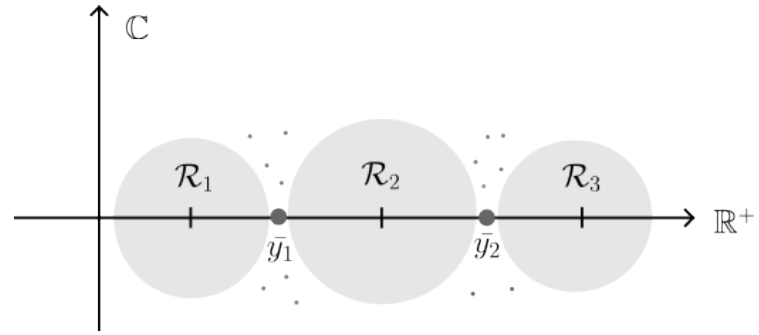
\includegraphics[width=0.55\linewidth]{Immagini/regioni di LY.png}
    \caption{esempio di sistema che può assumere tre fasi distinte associate alle regioni $\region$ rispettive.}
    \label{fig: regioni di LY}
\end{figure}
Al variare di $T$ può accadere per un certo valore critico $T_c$ che una radice lasci l'asse reale positivo; se ad esempio questo accade con $\bar{y}_1$, le regioni $\region_1$ e $\region_2$ si uniscono rimuovendo la possibilità di transizione al sistema tra le fasi associate ad esse. 

Ci si concentri adesso sul limite $V \to \infty$. Il teorema \eqref{teo: I teo LY} implica che la pressione  rimane continua anche nei punti corrispondenti alle radici $\bar{y}_i$ di $Q$, ma il secondo teorema \eqref{teo: II teo LY} si applica separatamente alle regioni $\region$ e pertanto la densità in generale non è continua in tali punti. Quindi, fissare dei valori di $y$ corrisponde a fissare dei valori per il potenziale chimico e la situazione che si presenta è del tipo mostrata in figura \ref{fig: andamento p(y) e p(v) (LY)}: invertendo la relazione tra la densità $1/v$ e $y$ segue un digramma $(p,V)$ a temperatura fissata che mostra delle transizioni di fase. 
\begin{figure}[h]
    \centering
    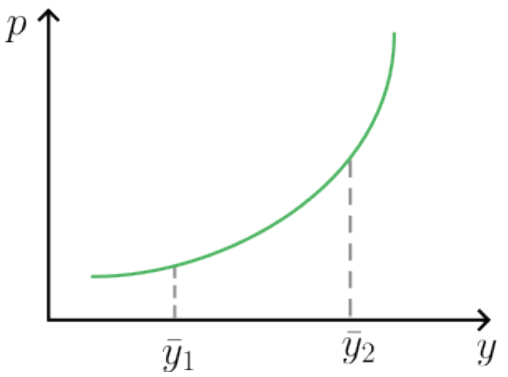
\includegraphics[width=0.3\linewidth]{Immagini/andamento p(y) (LY) 1.png}
    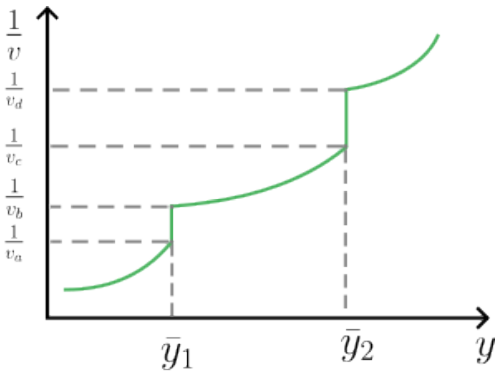
\includegraphics[width=0.3\linewidth]{Immagini/andamento p(y) (LY) 2.png}
    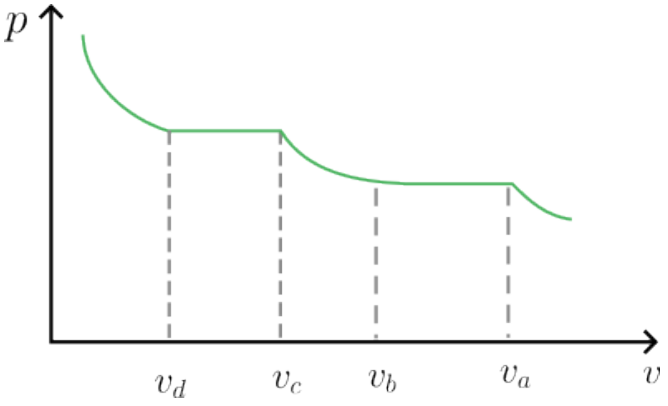
\includegraphics[width=0.35\linewidth]{Immagini/andamento p(v) (LY).png}
    \caption{andamento: (i) di $p$ in funzione di $y$; (ii) di $1/v$ in funzione di $y$; di $p$ in funzione di $v$.}
    \label{fig: andamento p(y) e p(v) (LY)}
\end{figure}
Si nota che in ogni regione $\region_i$ la particolare equazione di stato determina un altrettanto particolare espressione di $y \equiv y(T,V,N)$ e quindi di $\mu \equiv \mu(T,V,N)$, quando il potenziale chimico è considerato come variabile indipendente. Nei punti $\bar{y}_i$ corrispondenti alle transizioni i potenziali chimici coincidono, che è esattamente quanto richiesto dalla condizione per la coesistenza di fasi diverse \eqref{eq: condizione coesistenza}. 
\begin{obs}
    Lee e Yang hanno mostrato rigorosamente che questo meccanismo nel caso del ``lattice gas model'' è isomorfo al modello di Ising.
\end{obs}

\subsection{Transizioni continue del secondo ordine}
In Termodinamica, si è insistito in particolare sulle transizioni di fase del primo ordine tra due fasi che differiscono qualitativamente in modo profondo, come fase solida e liquida. Tuttavia, sono estremamente interessanti in vari ambiti anche le transizioni continue, in particolare in quelle del secondo ordine, come quella che avviene al punto critico dell'acqua. In queste transizioni i concetti chiave sono quelli di ``rottura spontanea di simmetria'' e di ``parametro d'ordine''. L'hamiltoniana microscopica è invariante rispetto ad un gruppo di simmetria $G$, che potrebbe essere ad esempio il gruppo delle rotazioni. Quello che succede per queste transizioni tipicamente è che:
\begin{enumerate}
    \item per $T > T_c$, lo stato macroscopico del sistema è invariante sotto trasformazioni di $G$ e si trova pertanto nella ``fase disordinata'' dove la simmetria è completamente conservata;
    \item per $T < T_c$, lo stato macroscopico del sistema è invariante sotto trasformazioni di un sottogruppo $G' \le G$ detto ``gruppo di stabilità'' e si trova pertanto ``fase ordinata'' dove avviene una rottura spontanea della simmetria. 
\end{enumerate}
Invece, un parametro d'ordine è una qualsiasi osservabile $O$ invariante sotto $G$ e che quindi ha valore medio nullo nella fase disordinata $\vmedio{O}_{D} = 0$, ma con valore medio non nullo nella fase ordinata $\vmedio{O}_O \neq 0$, il quale indica la rottura della simmetria.

\subsubsection{Transizione ferromagnetica}
Un esempio di rottura di simmetria è dato dalla transizione da ferromagnete a paramagnete alla temperatura critica di Curie $T_c$, in assenza di campo magnetico esterno. In questo caso il parametro d'ordine è la magnetizzazione $\vM$ che, essendo un vettore, in assenza di una direzione privilegiata il suo valore di aspettazione deve essere uguale a zero. Invece, quando avviene una rottura di simmetria e si ha una direzione privilegiata, non si ha più invarianza per rotazioni, ma solo rispetto al sottogruppo $SO(2)$. 
\begin{figure}[h]
    \centering
    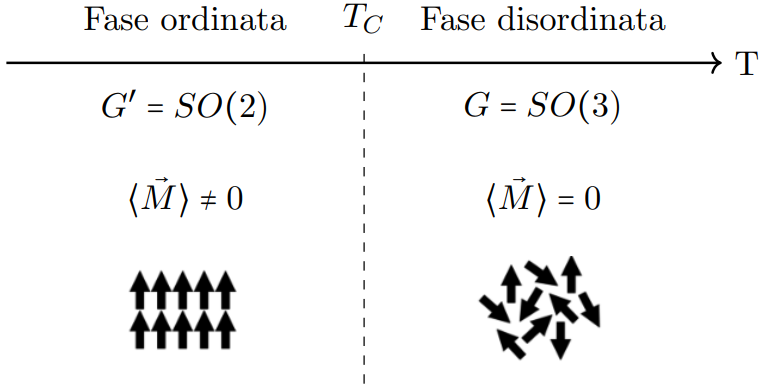
\includegraphics[width=0.53\linewidth]{Immagini/confronto fase ordinata - disordinata.png}
    \caption{confronto tra la fase ordinata e quella disordinata, con gruppi di simmetria relativi.}
    \label{fig: confronto fase ordinata - disordinata}
\end{figure}
\begin{obs}
    Una rappresentazione drasticamente semplificata dei sistemi ferromagnetici reali è data dal modello di Ising, il quale riesce a catturare comunque gli aspetti essenziali; in particolare, esso esibisce esplicitamente la transizione di fase ferromagnetica.
\end{obs}

\subsubsection{Proprietà di universalità}
Il fatto che anche un modello molto semplificato come quello di Ising catturi correttamente le caratteristiche di questa transizione continua del secondo ordine è legato al concetto di universalità, riguardante il comportamento del sistema nel limite per $T \to T_c$. Si definisce la temperatura ridotta $t$ come
\begin{equation}
    t := \frac{T - T_c}{T_c},
\end{equation}
la quale quantifica la vicinanza di $T$ alla temperatura critica $T_c$. Nelle transizioni del secondo ordine, le quantità termodinamiche seguono delle leggi di potenza per $|t| \to 0$; ad esempio, per la transizione ferromagnetica, avvicinandosi a $T_c$ dalla fase ordinata, ossia con $T < T_c$ e $t < 0$, la magnetizzazione spontanea $M \equiv \vmedio{\vM}$ tende a zero secondo 
\begin{equation}
\label{eq: legge di potenza magnetizzazione}
    M \propto (-t)^\beta.
\end{equation}
\begin{notz}
    In questo contesto, il parametro $\beta$ in \eqref{eq: legge di potenza magnetizzazione} non ha nulla a che fare con il parametro $\beta = 1/kT$.
\end{notz}
Invece, la suscettività magnetica $\chi$ e il calore specifico $c_{V}$ divergono secondo
\begin{equation}
\label{eq: legge di potenza suscettività e calore specifico}
    \chi \propto |t|^{-\gamma},\quad c_V \propto |t|^{-\alpha}.
\end{equation}
Gli esponenti $\alpha$, $\beta$ e $\gamma$ prendono il nome di ``indici critici'' e caratterizzano il comportamento del sistema nei pressi del punto critico; inoltre, non dipendono dai dettagli del sistema, ma da caratteristiche generali come i pattern di rottura di simmetria che provocano la riduzione $G \to G'$ e la dimensionalità $D$ dello spazio. Queste caratteristiche generali determinano classi di universalità dei sistemi fisici, i quali possono essere tra loro molto diversi come composizione microscopica, caratterizzata da un certo insieme di indici critici.

\section{Modello di Ising}
Nei materiali ferromagnetici reali gli atomi formano un reticolo più o meno regolare e sono dotati di spin, quindi di un momento magnetico $\bm{\mu}_B$. Tali momenti magnetici interagiscono fra di loro e percepiscono anche l'influenza di un campo magnetico esterno di intensità $B$. Nel modello semplificato si può assumere che:
\begin{enumerate}
    \item il reticolo è regolare, considerabile normalmente un ipercubo;
    \item ad ognuno degli $N$ siti reticolari è associata una variabile dinamica $s_i = \pm 1$, con $i = 1,\dots,N$, che rappresenta i due possibili autovalori della terza componente di $\mu_B$, se lo spin è pari ad $1/2$;
    \item un microstato del sistema corrisponde ad assegnare un insieme di variabili $\{s_i\}$ e il numero di possibili microstati $n$ è pari a $n = 2^N$, dato che in ogni sito si hanno due possibili scelte;
    \item due momenti magnetici $s_i$ ed $s_j$ interagiscono solo se $\vmedio{ij}$ è un ``link'', ossia solo se i due momenti sono primi vicini nel reticolo;
    \item le variabili $s_i$ interagiscono anche con un campo magnetico esterno $B$ presente in ogni punto tramite $h = \mu_BB$;
    \item l'hamiltoniana del modello è 
    \begin{equation}
    \label{eq: hamiltoninana modello di Ising}
        H = -J\sum_{\vmedio{ij}}s_is_j - h\sum_{i=1}^Ns_i,
    \end{equation}
    dove $J$ è il parametro macroscopico che determina l'intensità dell'accoppiamento tra gli spin primi vicini e il secondo termine di interazione tende ad allineare gli spin con il campo magnetico $B$ esterno;
    \item per descrivere un materiale ferromagnetico si pone $J > 0$.
\end{enumerate}
L'energia interna è più bassa se in un link $\vmedio{ij}$ i due spin $s_i$ ed $s_j$ sono concordi, cioè se $s_is_j = 1$; quindi, l'allineamento reciproco degli spin è favorito energeticamente e il secondo termine dell'hamiltoninana \eqref{eq: hamiltoninana modello di Ising} favorisce l'allineamento degli spin con il campo $h$. Essenzialmente, l'hamiltoniana fa tendere il sistema alla fase ordinata allineando tutti gli spin, mentre l'entropia svolge il ruolo opposto favorendo il disordine. Lo stato fondamentale di minima energia corrisponde a:
\begin{enumerate}
    \item quello in cui $s_i = 1$ per ogni $i$, se $h > 0$;
    \item quello in cui $s_i = -1$ per ogni $i$, se $h < 0$;
\end{enumerate}
Chiaramente, in assenza del campo esterno $h$ si hanno stati di energia minima sia che gli $s_i$ siano tutti allineati ``up'', cioè con $s_i = 1$, sia che siano tutti allineati ``down'', cioè con $s_i = -1$; per cui se $h = 0$ lo stato fondamentale è degenere. 

La funzione di partizione è data dalla somma su tutte le configurazioni, ossia su tutte le possibili scelte della variabile dinamica $s_i$ in ogni sito del reticolo, quindi
\begin{equation}
    Z = \sum_{\{s_i\}}e^{-\beta H(\{s_i\})}.
\end{equation}
Le variabili di controllo, oltre il numero di siti $N$ che viene tenuto fissato, sono la temperatura $T$ e il campo esterno $h$, entrambe intensive. Siccome il modello è definito su un reticolo, il volume $V$ non assume alcun ruolo. Ponendo $Z \equiv Z(T,h,N) = e^{-\beta G(T,h,N)}$, la funzione $G$ rappresenta, nel limite termodinamico, il potenziale appropriato alla scelta dell'insieme di variabili di controllo $\{T,h,N\}$, da non confondere con l'energia di Gibbs, anche se ci assomiglia. La variabile estensiva coniugata al campo $h$ è la magnetizzazione totale $M$, ottenuta a partire da $G$ tramite
\begin{equation}
\label{eq: magnetizzazione come media spin}
    \begin{split}
        M = -\frac{\p G}{\p h}\bigg|_{T,N} = \frac{1}{\beta}\frac{\p}{\p h}(\log{Z})\bigg|_{T,N} &= \frac{1}{\beta Z}\frac{\p}{\p h}\sum_{\{s_i\}}e^{-\beta H} \\
        &= -\frac{1}{Z}\sum_{\{s_i\}}\frac{\p H}{\p h}e^{-\beta H} \\
        &= \sum_{\{s_i\}}\bigg(\sum_{i=1}^N s_i\bigg)\frac{e^{-\beta H(\{s_i\})}}{Z} \\
        &= \bigvmedio{\sum_{i=1}^N s_i},
    \end{split}
\end{equation}
la quale quindi corrisponde al valore medio della somma degli spin $s_i$.

\subsubsection{Simmetria $\Z_2$}
Si consideri il caso in cui $h = 0$, l'hamiltoniana si riduce a $H = -J\sum_{\vmedio{ij}}s_is_j$ ed è invariante sotto trasformazioni di parità
\begin{equation}
    \Pi : s_i \longrightarrow -s_i,\quad \forall i.
\end{equation}
Questa operazione definisce il gruppo di simmetria $\Z_2$ dato che applicare due volte una trasformazione di parità restituisce l'oggetto iniziale, in termini operatoriali $\Pi^2 = \MI$. L'osservabile $\sum_is_i$ rappresenta un parametro d'ordine, infatti essa non è invariante sotto l'azione di $\Z_2$ in quanto 
\begin{equation}
    \Pi : \nsum_is_i \longrightarrow -\bigg(\nsum_is_i\bigg).
\end{equation}
Quindi, il valore medio $M = \vmedio{\nsum_is_i}$ non nullo indica una rottura della simmetria del gruppo $\Z_2$, spontanea perché invece l'hamiltoniana è invariante sotto l'azione di tale gruppo come detto prima. Se il numero $N$ di siti reticolari è finito, la rottura spontanea di simmetria non può avvenire, in quanto $s_i = \pm 1$ e sommare su tutte le possibili configurazioni degli $s_i$ o dei $\tilde{s}_i \equiv -s_i$ è del tutto equivalente. Pertanto, si può scrivere la relazione
\begin{equation}
    M = \sum_{\{s_i\}}\bigg(\sum_{i=1}^N s_i\bigg)\frac{e^{-\beta H(\{s_i\})}}{Z} = \sum_{\{\tilde{s_i}\}}\bigg(-\sum_{i=1}^N \tilde{s_i}\bigg)\frac{e^{-\beta H(\tilde{s_i})}}{Z},
\end{equation}
da cui, notando che le variabili $\{\tilde{s}_i\}$ sono mute essendo sono sommate, si può richiamare $\tilde{s}_i \to s_i$ e trovare che
\begin{equation}
    M = \sum_{\{s_i\}}\bigg(\sum_{i=1}^N s_i\bigg)\frac{e^{-\beta H(\{s_i\})}}{Z} = -\sum_{\{s_i\}}\bigg(\sum_{i=1}^N s_i\bigg)\frac{e^{-\beta H(\{s_i\})}}{Z} = -M,
\end{equation}
per cui necessariamente
\begin{equation}
    M  = 0.
\end{equation}
Quindi, le manipolazioni eseguite nel caso di $N$ finito sono sicuramente valide in quanto si ha a che fare con somme finite; invece, nel limite termodinamico, sorgono problemi riguardanti le condizioni al contorno e di convergenza che in linea di principio possono invalidare tali manipolazioni e permettere la comparsa di una fase ordinata in cui la simmetria $\Z_2$ viene rotta rendendo $M \neq 0$. Tutto ciò è analogo a quanto è emerso dalla teoria di Lee - Yang: le transizioni di fase sono legate a punti di non analiticità della funzione di partizione, siccome i singoli addendi della funzione di partizione sono analitici in $\beta$, tale è anche la loro somma, a meno che vi siano infiniti addendi e la somma diventi una serie.

Analogamente, in presenza del campo esterno $h$, la simmetria di $\Z_2$ mappa il modello microscopico in un modello per il campo $-h$, ovvero adesso
\begin{equation}
    H(\{s_i\},h) =  H(\{\tilde{s}_i\},-h).
\end{equation}
Dato che continua a valere l'equivalenza sulle operazioni di somma $\sum_{\{s_i\}} = \sum_{\{\tilde{s}_i\}}$, questo implica che
\begin{equation}
    Z(T,h,N) = Z(T,-h,N),\quad G(T,h,N) = G(T,-h,N),
\end{equation}
mentre per la magnetizzazione che
\begin{equation}
    M(T,h,N) = - M(T,-h,N).
\end{equation}
Il modello di Ising per quanto semplificato, cattura l'essenza della rottura spontanea di simmetria $\Z_2$. Si vedrà infatti che esso prevede, per reticoli in dimensione $D > 1$, la transizione di fase ferromagnetica e la presenza di una fase ordinata, date le proprietà di universalità delle transizioni di fase del secondo ordine.

\section{Lattice gas model}
Il modello di Ising è isomorfo al modello semplificato ``lattice gas model'' per un gas classico interagente, usato come punto di partenza per lo studio delle transizioni gas-liquido. Sia $V$ il volume occupato dal gas e lo si suddivida in $N$ celle elementari di volume $v_0$. Si ipotizza che questo gas non sia libero, ma sia caratterizzato da un potenziale di interazione intermolecolare che non permetta la sovrapposizione tra le particelle, come quello usato nella \eqref{eq: potenziale Lennard-Jones approx.}. Quindi, ogni cella può essere occupata al più da una singola particella di volume $v_0$ e il volume totale $V$ occupato dal gas si può esprimere come $V = Nv_0$. Si suppone inoltre che il potenziale di interazione risulti attrattivo per particelle molto vicine. In questa trattazione estremamente approssimata si trascura l'energia cinetica delle particelle, per cui il modello va applicato per temperature non eccessivamente alte, risultando non particolarmente adeguato a descrivere il sistema nel limite classico. 

Nell'ensemble grancanonico, il numero di particelle $N_p$ può fluttuare e ogni microstato $\nu$ corrisponde alla collezione di numeri di occupazione $\{n_i\}$ con $n_i = 0,1$ per $i = 1,\dots,N$. All'energia totale contribuiscono solo le particelle in celle continue, ossia prime vicine, quindi l'energia e il numero di particelle del microstato $\{n_i\}$ sono date da
\begin{equation}
    E(\{n_i\}) = -\epsilon\sum_{\vmedio{ij}}n_in_j,\quad N_p(\{n_i\}) = \sum_{i=1}^Nn_i.
\end{equation}
Pertanto, la funzione di partizione grancanonica è
\begin{equation}
\label{eq: funzione di partizione lattice gas model (grancanonico)}
    Q(T,V,\mu) = \sum_{\{n_i\}}\exp{\bigg(\beta\epsilon\sum_{\vmedio{ij}}n_in_j + \beta\mu\sum_{i=1}^Nn_i\bigg)}.
\end{equation}
La corrispondenza tra il lattice gas model e il modello di Ising si può esprimere graficamente come in figura \ref{fig: relazione lattice gas model ed Ising}. 
\begin{figure}[h]
    \centering
    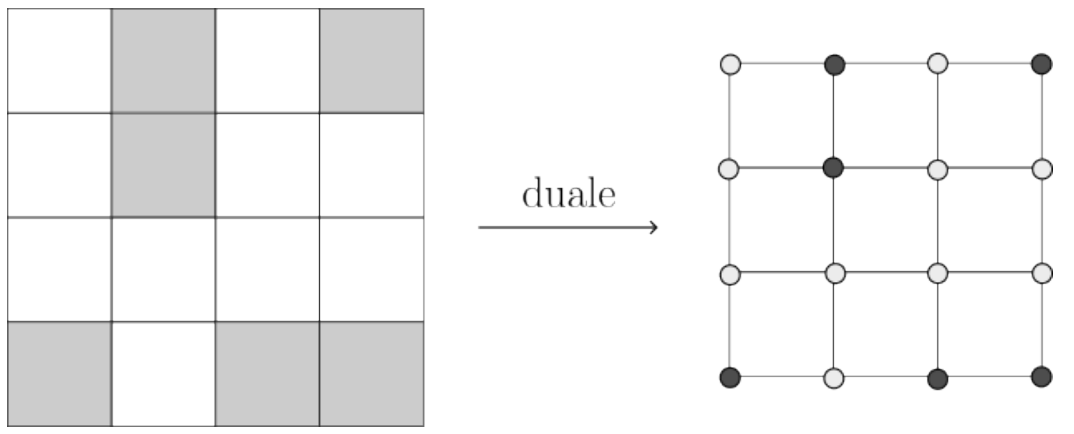
\includegraphics[width=0.7\linewidth]{Immagini/relazione lattice gas model ed Ising.png}
    \caption{corrispondenza tra il lattice gas model ed il modello di Ising.}
    \label{fig: relazione lattice gas model ed Ising}
\end{figure}
Tutte le configurazioni degli $n_i$ si possono mappare in configurazione del modello di Ising prendendo il modello duale a quello delle celle facendo corrispondere $n_i = 1 \to s_i = 1$ e $n_i = 0 \to s_i = -1$, esplicitamente
\begin{equation}
\label{eq: I corrispondenza LGM e MI}
    s_i = 2n_i - 1\quad\longleftrightarrow\quad n_i = \frac{s_i + 1}{2}.
\end{equation}
Rispetto a questa corrispondenza, l'esponente nella funzione di partizione \eqref{eq: funzione di partizione lattice gas model (grancanonico)} diventa
\begin{equation}
    \begin{split}
        \beta\epsilon\sum_{\vmedio{ij}}n_in_j + \beta\mu\nsum_in_i &= \beta\bigg[\frac{\epsilon}{4}\sum_{\vmedio{ij}}s_is_j + \bigg(\frac{\epsilon q}{2} + \frac{\mu}{2}\bigg)\sum_{i=1}^Ns_i + N\bigg(\frac{\epsilon q}{8} + \frac{\mu}{2}\bigg)\bigg] \\
        &= \beta H + \mathrm{costante},
    \end{split}
\end{equation}
dove $H$ è l'hamiltoniana del modello di Ising \eqref{eq: hamiltoninana modello di Ising} con parametri
\begin{equation}
\label{eq: II corrispondenza LGM e MI}
    J = \frac{\epsilon}{4},\quad h = \frac{1}{2}(\mu + \epsilon q),
\end{equation}
dove $q$ è il ``numero di coordinazione'' del reticolo, ossia il numero di siti primi vicini di un dato sito. Quindi, la differenza tra i due modelli corrisponde quindi ad una traslazione di una costante. Quest'ultima è indipendente dal microstato ed è irrilevante dato che viene riassorbito dalla normalizzazione della funzione di partizione non influenzando quindi la probabilità dei microstati e i valori medi delle osservabili. Dunque, il lattice gas model e il modello di Ising, con le corrispondenze \eqref{eq: I corrispondenza LGM e MI} e \eqref{eq: II corrispondenza LGM e MI}, sono equivalenti, ossia isomorfi. In particolare, vale l'equivalenza sulle operazioni di somma $\sum_{\{n_i\}} = \sum_{\{s_i\}}$, dato che le configurazioni sono mappate uno ad uno, quindi
\begin{equation}
    Q(T,V,\mu) = \mathrm{costante}\times Z(T,h,N).
\end{equation}
Inoltre, il numero medio di particelle nel lattice gas model è dato da
\begin{equation}
    \vmedio{N_p} = \bigvmedio{\sum_{i=1}^Nn_i} = \frac{1}{2}\bigvmedio{\sum_{i=1}^N(s_i + 1)} = \frac{M + N}{2}.
\end{equation}
La comparsa della magnetizzazione nel modello di Ising corrisponde, nel lattice gas model, ad una condensazione delle particelle in una fase liquida e quindi ad una transizione di fase. 

\section{Modello di Ising 1-dimensionale}
Il caso unidimensionale del modello di Ising è quello più semplice dove è possibile risolvere esattamente la funzione di partizione. Purtroppo, è anche il caso meno interessante dato che non mostra transizioni di fase: ogni spin ha troppi pochi primi vicini e quindi l'ordine non riesce a comparire con il disordine dovuto all'entropia. 
\begin{figure}[h]
    \centering
    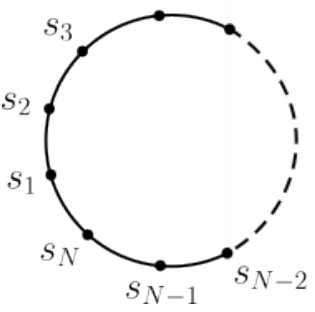
\includegraphics[width=0.25\linewidth]{Immagini/modello Ising D = 1.png}
    \caption{reticolo unidimensionale con condizione periodiche al contorno.}
    \label{fig: modello Ising D = 1}
\end{figure}
Come punto di partenza, si considera  un reticolo unidimensionale rappresentabile come una ``catena'' di spin; poi, si impongono delle condizioni al contorno periodiche\footnote{Si scelgono qui condizioni al contorno periodiche solamente per una questione di semplicità, ma in generale si possono usare anche altre condizioni al contorno senza particolari problemi.} rendendo così la catena chiusa con $s_1$ e $s_N$ primi vicini soddisfacenti la relazione $s_1 = s_{N+1}$, come si vede in figura \ref{fig: modello Ising D = 1}. Quindi, la funzione di partizione è data
\begin{equation}
    \begin{split}
        Z &= \sum_{\{s_i\}}\exp\bigg(\beta J\sum_{\vmedio{ij}}s_is_j + \beta h\sum_{i=1}^Ns_i\bigg) \\
        &= \sum_{\{s_i\}}\exp\bigg[\beta J\sum_{i=1}^Ns_is_{i+1} + \frac{\beta h}{2}\bigg(\sum_{i=1}^Ns_i + \sum_{i=1}^Ns_{i+1}\bigg)\bigg],
    \end{split}
\end{equation}
dove si è riscritto in modo simmetrico il secondo termine all'esponente e da cui si deduce che la struttura della catena implica
\begin{equation}
    \sum_{\vmedio{ij}}s_is_j = \sum_{i=1}^Ns_is_{i+1}.
\end{equation}
In questo modo si ha
\begin{equation}
    \begin{split}
        Z &= \sum_{\{s_i\}}\prod_{i=1}^N\exp{\bigg(\beta Js_is_{i+1} + \frac{\beta h}{2}s_i + \frac{\beta h}{2}s_{i+1}\bigg)} \\
        &= \sum_{\{s_i\}}\prod_{i=1}^N\TM_{s_i,s_{i+1}} \\
        &= \sum_{s_1,\dots,s_N}\underbrace{\TM_{s_1,s_2}\TM_{s_2,s_3}}_{=\TM^2_{s_1,s_3}}\cdots\TM_{s_{N-1},s_N}\TM_{s_N,s_1} \\
        &= \Tr{\TM^N},
    \end{split} 
\end{equation}
dove si è sfruttata la periodicità della catena e si è introdotta la ``matrice di trasferimento'' del sistema $\TM \equiv \TM_{s_i,s_{i+1}}$ definita come 
\begin{equation}
    \TM := 
    \begin{pmatrix}
        e^{\beta J + \beta h} & e^{-\beta J} \\
        e^{-\beta J} & e^{\beta J - \beta h}
    \end{pmatrix},
\end{equation}
la quale lega i possibili valori di un sito $s_i$ con i possibili valori di quello successivo $s_{i+1}$. La matrice $\TM$ può essere diagonalizzata risolvendo l'equazione caratteristica $\det{(\TM - \lambda\MI)} = 0$ che fornisce gli autovalori 
\begin{equation}
\label{eq: autovalori matrice trasferimento}
    \lambda_\pm = e^{\beta J}(\cosh{\beta h} \pm \sqrt{\cosh^2{(\beta h)} - 2e^{-2\beta J}\sinh{2\beta J}},\quad \lambda_+ > \lambda_-.
\end{equation}
Pertanto, la matrice di trasferimento è
\begin{equation}
    \TM^N = 
    \begin{pmatrix}
        \lambda_+^N & 0 \\
        0 & \lambda_-^N
    \end{pmatrix},
\end{equation}
per cui la funzione di partizione è
\begin{equation}
\label{eq: funzione di partizione Ising D=1}
    Z = \lambda_+^N + \lambda_-^N = \lambda_+^N\bigg[1 + \bigg(\frac{\lambda_-}{\lambda_+}\bigg)^N\bigg],
\end{equation}
che nel limite termodinamico si riduce semplicemente all'autovalore di $\TM$ maggiore
\begin{equation}
\label{eq: funzione di partizione Ising D=1 (limite TD)}
    Z \simeq \lambda_+^N,\quad N \to \infty.
\end{equation}
L'energia libera $G$, sempre in questo limite, è data da
\begin{equation}
    \begin{split}
        G &= -\frac{\log{Z}}{\beta} \\
        &=-N\bigg[J + \frac{1}{\beta}\log{\bigg(\cosh{\beta h} + \sqrt{\cosh^2{(\beta h)} - 2e^{-2\beta J}\sinh{2\beta J}}\bigg)}\bigg],
    \end{split}
\end{equation}
da cui si calcola la magnetizzazione
\begin{equation}
    M = -\frac{\p G}{\p h}\bigg|_{T,N} =  \frac{N\sinh{\beta h}}{\sqrt{\cosh^2{(\beta h)} - 2e^{-2\beta J}\sinh{2\beta J}}}.
\end{equation}
Se è presente un campo esterno, allora si genera una magnetizzazione, invece in assenza di questo, per $T \neq 0$, è sempre vera in $D = 1$ l'implicazione 
\begin{equation}
    h = 0\quad\Longrightarrow\quad M = 0.
\end{equation}
La magnetizzazione spontanea è sempre nulla e si è sempre nella fase disordinata in cui la simmetria di $\Z_2$ è conservata. Tuttavia, per reticoli $D$-dimensionali con $D > 1$ compare la transizione ferromagnetica, che non appare nel caso $1$-dimensionale a causa dell'influenza soppressa dei termini di accoppiamento che tendono ad allineare il sistema in quanto ogni sito ha solo due primi vicini. Sempre nel caso in cui $h = 0$, l'espressione esatta della funzione di partizione è un sottocaso dell'espressione generale \eqref{eq: funzione di partizione Ising D=1} con $\lambda_\pm$ dati dalla \eqref{eq: autovalori matrice trasferimento} che in assenza di campo esterno sono
\begin{equation}
    \lambda_+ = 2\cosh{\beta J},\quad \lambda_- = 2\sinh{\beta J},
\end{equation}
per cui la funzione di partizione è
\begin{equation}
    Z = (2\cosh{\beta J})^N + (2\sinh{\beta J})^N,
\end{equation}
da cui, trascurando nel limite termodinamico il secondo termine, si trova che l'energia libera vale
\begin{equation}
    G \simeq -\frac{N}{\beta}\log{(2\cosh{\beta J})},
\end{equation}
che per $T > 0$ è una funzione analitica, ossia priva di singolarità in $G$ e nelle sue derivate, pertanto non si presentano transizioni di fase. 
\begin{obs}
    Il modello di Ising 1-dimensionale con $h = 0$ può venire facilmente risolto anche con metodi diversi da quello della matrice di trasferimento. Tali metodi possono essere impiegati anche in dimensionalità $D$ generica e forniscono informazioni importanti anche se l'unico caso risolvibile esattamente, anche con $h = 0$, rimane quello bidimensionale.
\end{obs}

\section{Sviluppo ad alta temperatura per \texorpdfstring{$D = N$}{D = N}}
La tecnica che segue è applicabile quando il modello di Ising è definito tramite un qualsiasi grafo $G$, ossia su qualsiasi reticolo avente $N$ siti ai quali sono associate le variabili $s_i$ e $L$ link $\vmedio{ij}$ che collegano i siti continui, ossia i primi vicini. Se il reticolo è regolare, ossia se in ogni sito entra lo stesso numero $q$ di link, si ha che il numero di link è pari a
\begin{equation}
    L = \frac{Nq}{2},
\end{equation}
dove per ogni sito si sono considerati tutti i suoi primi vicini e si è diviso per due in modo da evitare di contare troppi link, ovviamente a parte per i siti sul bordo dato che possono avere un numero minore di primi vicini. Ad ogni link $\vmedio{ij}$ viene associato il fattore
\begin{equation}
\label{eq: identità sviluppo alta T}
    e^{\beta Js_is_j} \equiv e^{Ks_is_j},\quad K \equiv \beta J.
\end{equation}
Quindi, ciò che determina l'intensità dell'interazione nella funzione di partizione è un rapporto adimensionale tra l'energia di interazione e l'energia termica. Inoltre, vale l'identità
\begin{equation}
\label{eq: relazione exp(Ksisj) e cosh(K)}
    \begin{split}
        e^{Ks_is_j} = \cosh{K}(1  + s_is_j\tanh{K}) \equiv \cosh{K}(1  + s_is_jv),\quad v \equiv \tanh{K}.
    \end{split}
\end{equation}
Per considerare il limite di alta temperatura si assume $K \ll 1$, inoltre si prende $h = 0$ per semplicità, quindi la funzione di partizione è
\begin{equation}
    \begin{split}
        Z = \sum_{\{s_i\}}\exp{\bigg(K\sum_{\vmedio{ij}}s_is_j\bigg)} = \sum_{\{s_i\}}\prod_{\vmedio{ij}}e^{Ks_is_j} &= \sum_{\{s_i\}}\prod_{\vmedio{ij}}[\cosh{K}(1  + s_is_jv)] \\
        &= \cosh^L{(K)}\sum_{\{s_i\}}\prod_{\vmedio{ij}}(1  + s_is_jv).
    \end{split}
\end{equation}
Il prodotto sui link $\prod_{\vmedio{ij}}(1  + s_is_jv)$ è uno sviluppo che contiene $2^L$ termini, infatti si hanno due termini per ogni link: il termine dato da $1$ e quello con $v$; di questi può essere data una rappresentazione grafica tramite la notazione per i due possibili contributi del link $\vmedio{ij}$ in figura \ref{fig: notazione grafica prodotto link}. L'espansione del prodotto corrisponde all'espansione nei possibili sottografi di link attivi. 
\begin{figure}[h]
    \centering
    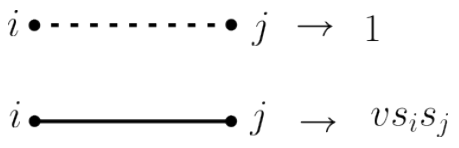
\includegraphics[width=0.35\linewidth]{Immagini/notazione grafica prodotto link.png}
    \caption{rappresentazione grafica dei termini del prodotto sui link: (i) link vuoto; (ii) link attivo.}
    \label{fig: notazione grafica prodotto link}
\end{figure}
\begin{ex}
    Se $G$ è un catena chiusa 1-dimensionale con $N = 3$ e $L = 3$, allora ci sono $2^3 = 8$ termini possibili, mostrati in figura \ref{fig: prodotto link con N = 3 ed L = 3 in D = 1}. Attraverso la somma dei triangoli si ottengono tutti i termini dello sviluppo; ad esempio, l'ultimo termine in figura corrisponde a tre link attivi per cui è dato da
    \begin{equation}
        (vs_1s_2)(vs_2s_3)(vs_3s_1) = v^3s_1s_2s_2s_3s_3s_1 = v^3,\quad s_i^2 = 1,\,i=1,2,3.
    \end{equation}
    \begin{figure}[H]
        \centering
        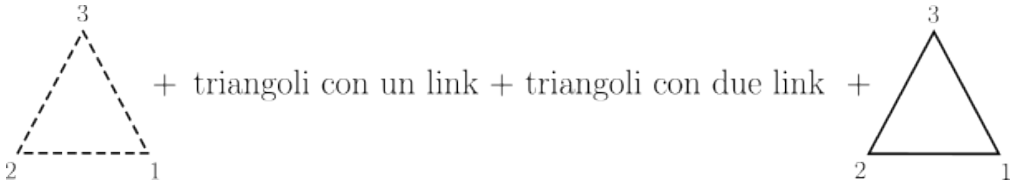
\includegraphics[width=0.75\linewidth]{Immagini/prodotto link con N = 3 ed L = 3 in D = 1.png}
        \caption{espansione del prodotto sui link per $N = 3$ ed $L = 3$ in $D = 1$.}
        \label{fig: prodotto link con N = 3 ed L = 3 in D = 1}
    \end{figure}
\end{ex}
Ci si concentri ora su un generico contributo di questa espansione. Nella funzione di partizione \eqref{eq: funzione di partizione Ising D=1} questo va sommato su tutti i possibili valori delle variabili $s_i$. Per un dato sito $i$, se $n_i$ è il numero di link attivi che entrano in tale sito, si ha la somma
\begin{equation}
    \sum_{s_i=\pm1}(s_i)^{n_i} = 
    \begin{cases}
        0,\quad n_i\ \mathrm{dispari} \\
        2,\quad n_i\ \mathrm{pari}\vee 0
    \end{cases}.
\end{equation}
Quindi, nella somma si devono scegliere i termini dello sviluppo in cui ogni variabile $s_i$ compare un numero pari di volte. Alla funzione di partizione contribuiscono dunque esclusivamente i sottografi in cui in ogni sito entra un numero pari di link attivi: tali configurazioni sono poligoni chiusi. Un dato poligono di lunghezza $l$, ossia contenente $l$ link attivi contribuisce con un termine pari a 
\begin{equation}
    2^Nv^l,
\end{equation}
infatti, in ogni sito del reticolo si ha un contributo pari a 2 poiché o non entrano link, e $n_i = 0$, o ne entra un numero pari, inoltre ad ogni link attivo si associa un contributo pari a $v$. Dunque, la funzione di partizione si può esprimere come
\begin{equation}
\label{eq: funzione di partizione Ising alta T}
    Z = 2^N\cosh^L{(K)}\sum_{l=0}^Lg_lv^l,
\end{equation}
dove $g_l$ è il numero di poligoni chiusi di lunghezza $l$ che possono essere tracciati sul grafo $G$. Il parametro di sviluppo $v$ è tale che $v \ll 1$ quando $\beta J \ll 1$, ossia quando $kT \gg J$. L'espressione \eqref{eq: funzione di partizione Ising alta T} costituisce quindi un'espansione perturbativa, valida per alte temperature\footnote{I passaggi eseguiti per arrivare a questa espressione sono concettualmente analoghi a quelli svolti per la cluster expansion del gas interagente; in effetti, l'espansione del modello di Ising corrisponde alla cluster expansion del lattice gas model.}.

\section{Sviluppo a bassa temperatura per \texorpdfstring{$D = N$}{D = N}}
I progressi verso la determinazione di una transizione di fase possono essere fatti grazie alla possibilità di organizzare la funzione di partizione in modo alternativo, tramite uno sviluppo nel limite di bassa temperatura e alle relazioni non banali di dualità che possono sussistere tra queste due espansioni. A tal proposito, si riconsideri la funzione di partizione 
\begin{equation}
    Z = \sum_{\{s_i\}}\prod_{\vmedio{ij}}e^{Ks_is_j}
\end{equation}
e si supponga che per un determinato microstato $\{s_i\}$ si abbia un numero $n$ di link $\vmedio{ij}$ per cui $s_is_j = -1$, corrispondente al numero di coppie di spin primi vicini antiparalleli. Quindi, il numero di link $\vmedio{ij}$ con spin paralleli, ossia tali che $s_is_j = 1$, è dato da $L - n$. Pertanto, si può esprimere il prodotto sui link come
\begin{equation}
    \prod_{\vmedio{ij}}e^{Ks_is_j} = (e^K)^{L-n}(e^{-K})^{n} = e^{KL}e^{-2nK},
\end{equation}
che è un'espansione in serie nel parametro $e^{-2K}$. Quindi, se si denota con $\tilde{g}_n$ il numero di configurazioni distinte in cui compaiono $n$ primi vicini con spin antiparalleli, la funzione di partizione si può scrivere come
\begin{equation}
\label{eq: funzione di partizione Ising bassa T}
    Z \equiv 2e^{KL}\nsum_n\tilde{g}_n\tilde{v}^n,\quad \tilde{v} \equiv e^{-2K},
\end{equation}
dove il fattore moltiplicativo 2 è dovuto al fatto che ogni configurazione con $n$ coppie di spin antiparallelo ammette due realizzazioni, collegate tra loro tramite la simmetria $\Z_2 : s_i \to -s_i,\,\forall i$, cioè dallo scambio di tutti gli spin up con quelli down e viceversa.  

Per considerare il limite di bassa temperatura si assume $K \gg 1$, inoltre si prende $h = 0$ per semplicità. Il parametro di sviluppo $\tilde{v}$ è tale che $\tilde{v} \ll 1$ quando $\beta J \gg 1$, ossia quando $kT \ll J$. Quindi, l'espressione \eqref{eq: funzione di partizione Ising bassa T} costituisce quindi un'espansione perturbativa, valida per basse temperature. Il primo termine con $n = 0$ richiede l'assenza di coppie di spin antiparallelo, per cui $\tilde{g}_0 = 1$ con le due realizzazioni mostrate in figura \ref{fig: realizzazioni energia minima}, corrispondenti ai due microstati degeneri di energia minima.
\begin{figure}[h]
    \centering
    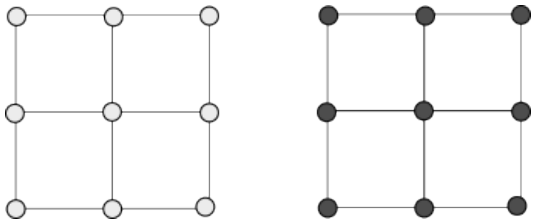
\includegraphics[width=0.4\linewidth]{Immagini/realizzazioni energia minima.png}
    \caption{realizzazioni corrispondenti ai microstati degeneri di energia minima.}
    \label{fig: realizzazioni energia minima}
\end{figure}
I termini successivi dello sviluppo sono via via più disordinati per l'introduzione di spin invertiti. Nel caso del reticolo quadrato in dimensione $D = 2$, l'inversione di uno spin, che può avvenire in qualsiasi degli $N$ siti, introduce quattro coppie di spin antiparallelo, come mostrato in figura \ref{fig: realizzazioni 1-flip e 2-flip}, per cui $\tilde{g}_1 = \tilde{g}_2 = \tilde{g}_3 = 0$ e $\tilde{g}_4 = N$. 
\begin{figure}[h]
    \centering
    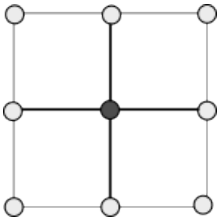
\includegraphics[width=0.2\linewidth]{Immagini/realizzazione 1-flip.png}
    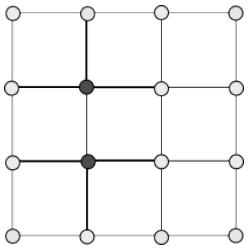
\includegraphics[width=0.2\linewidth]{Immagini/realizzazione 2-flip.png}
    \caption{realizzazione in seguito all'inversione dello spin di: (i) un sito; (ii) due siti.}
    \label{fig: realizzazioni 1-flip e 2-flip}
\end{figure}
Invece, non è possibile avere cinque coppie antiparallele, ma invertendo due spin primi vicini in uno degli $2N$ modi possibili diversi si possono ottenere sei coppie di spin antiparallelo, rappresentato sempre in figura \ref{fig: realizzazioni 1-flip e 2-flip}, insieme ovviamente alle configurazioni $\Z_2$ simmetriche rispetto a queste. Quindi, $\tilde{g}_5 = 0$, $\tilde{g}_6 = 2N$ e per questo particolare reticolo si ha
\begin{equation}
    \begin{split}
        Z &= 2e^{2NK}(1 + N\tilde{v}^4 + 2N\tilde{v}^6 + \cdots) \\
        &= 2e^{2NK}(1 + Ne^{-8K} + 2Ne^{-12K} + \cdots),\quad L = \frac{Nq}{2} = 2N.
    \end{split}
\end{equation}

\section{Argomento di Peierls}
La prima dimostrazione del fatto che il modello di Ising ammetta una fase ordinata in dimensione $D \ge 2$ è dovuta a Peierls. L'argomento di Peierls si applica nel limite termodinamico e permette di capire se ci si dovrebbe aspettare una transizione di fase o meno. Nel limite termodinamico, lo stato macroscopico del sistema all'equilibrio avrà energia libera $G$ minima. Una fase ordinata può esistere a patto che corrisponda ad un minimo stabile di $G$ rispetto alle fluttuazioni termiche, ovvero se queste ultime non abbassano l'energia libera. Quindi si deve vedere se le fluttuazioni termiche, in cui lo spin cambia di segno, alzano o abbassano l'energia libera rispetto alla configurazione ordinata. Ricapitolando, se $\Delta G \ge 0$, allora la fase è ordinata e $G$ permette un minimo stabile, al contrario se $\Delta G < 0$, allora il sistema è instabile.

\subsubsection{$\Delta G$ per il modello di Ising 1-dimensionale}
Partendo da uno stato completamente ordinato, mostrato in figura \ref{fig: variazione G D = 1}, si fissa un sito qualsiasi e ci si chiede se le fluttuazioni che portano a una configurazione in cui tale spin è invertito alzano o abbassano l'energia libera. 
\begin{figure}[h]
    \centering
    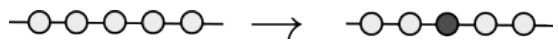
\includegraphics[width=0.5\linewidth]{Immagini/variazione G D = 1.png}
    \caption{inversione dello spin di un sito di un reticolo unidimensionale.}
    \label{fig: variazione G D = 1}
\end{figure}
La variazione di energia è $\Delta G=\Delta E-T\Delta S$. Nello stato iniziale l'energia è l'energia minima $E_0=-NJ$ (con condizioni periodiche perché ci sono $N$ link e sono tutti paralleli), mentre l'entropia è nulla in quanto c'è solo una configurazione possibile, per cui $S = k\log N_{\mathrm{config}} = k\log{1} = 0$.

Dato che alla variazione di energia $\Delta E$ contribuiscono solo i link che legano siti a spin antiparallelo, si ha una classe di configurazioni che corrispondono alla stessa $\Delta E$ dette ``isole di spin''. Le configurazioni in cui lo spin selezionato è invertito che hanno la minima variazione di energia sono quelle in cui si crea un'isola di spin invertiti, che comprende il sito scelto, come mostrato in figura \ref{fig: isola di spin D = 1}. Qualsiasi sia la lunghezza $L$ di tale isola, la variazione energetica rispetto allo stato ordinato è pari a
\begin{equation}
    \Delta E = 2 \times 2J = 4J
\end{equation}
perché si hanno ora due coppie contigue con spin antiparallelo per ciascuna delle quali il contributo all'energia è $J$ invece di $-J$.
\begin{figure}[h]
    \centering
    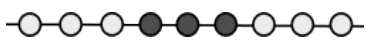
\includegraphics[width=0.35\linewidth]{Immagini/isola di spin D = 1.png}
    \caption{isola di spin in $D = 1$.}
    \label{fig: isola di spin D = 1}
\end{figure}

Vi sono $L$ modi di ``sistemare'' un'isola di lunghezza $L$ in modo che comprenda lo spin fissato\footnote{Ossia ci sono $L$ modi di sistemare il sito con spin invertito.}, per cui ora l'entropia non è nulla e si ha invece
\begin{equation}
    \Delta S = k \log L.
\end{equation}
Dunque, la variazione di energia libera è pari a 
\begin{equation}
    \Delta G = \Delta E - T \Delta S = 4J - kT \log L.
\end{equation}
Per qualsiasi $T>0$, si può trovare un valore di $L$ abbastanza grande da abbassare l'energia libera. Dunque, lo stato ordinato non è termodinamicamente stabile, per cui il modello unidimensionale non ammette una fase ordinata, come già dedotto dalla soluzione esatta, e non ci si aspetta una transizione di fase.

\subsubsection{$\Delta G$ per il modello di Ising 2-dimensionale}
Si consideri un'isola di spin invertiti che contenga un sito arbitrariamente scelto come fatto in figura \ref{fig: isola di spin D = 2}. 
\begin{figure}[h]
    \centering
    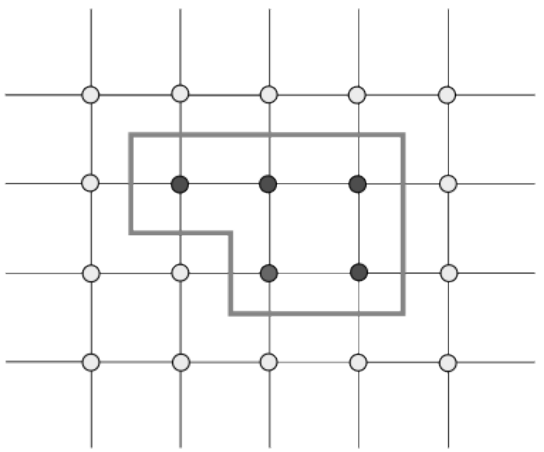
\includegraphics[width=0.35\linewidth]{Immagini/isola di spin D = 2.png}
    \caption{isola di spin in $D = 2$.}
    \label{fig: isola di spin D = 2}
\end{figure}
Si vogliono ora considerare tutte le fluttuazioni che invertono uno spin. Come prima cosa, si nota che il numero di coppie contigue con spin antiparallelo è pari al numero di link che attraversano il ``domain wall'' che racchiude l'isola. Introducendo quindi il reticolo duale, in cui vertici sono nel centro delle facce del reticolo originario, se il domain wall è un poligono fatto di $L$ segmenti (in figura \ref{fig: isola di spin D = 2} $L = 10$), nel reticolo duale essa è attraversata da $L$ links del reticolo originario, per cui
\begin{equation}
    \Delta E = 2JL,
\end{equation}
poiché si ha una variazione di $2J$ per ogni coppia con spin antiparallelo. Il numero di spin invertiti coincide con l'area $A(L)$ della regione circondata dal domain wall, cioè il numero di facce del reticolo duale contenute all'interno del domain wall. Non si conosce in generale il valore preciso dell'area, perché può avere forme diverse, ma sicuramente si può scrivere che
\begin{equation}
    A \le \bigg(\frac{L}{2\pi}\bigg)^2 \le \frac{L^2}{4\pi},
\end{equation}
in quanto deve essere minore o uguale alla figura con l'area maggiore, corrispondente ad un cerchio di raggio $L/2\pi$. Inoltre si possono avere diverse ``forme'' $\sigma(L)$ dell'isola, per le quali si può affermare che
\begin{equation}
    \sigma(L) \le 3^L,
\end{equation}
dato ad ogni ``passo'' ci si può muovere in tre direzioni; tuttavia, questa è una stima superiore perché non tutte le scelte sono libere, dato che la curva deve chiudersi. In definitiva, il numero di configurazioni $W(L)$, che consiste in isole di spin invertiti che creano $L$ coppie di spin antiparallelo è dato da
\begin{equation}
    W(L) \le 3^L\frac{L^2}{4\pi},
\end{equation}
da cui si ricava che la variazione di entropia è
\begin{equation}
    \Delta S = k\log{W(L)} \le kL\ln3 + \mathcal{O}(\log{L}),
\end{equation}
per cui la variazione di energia libera risulta essere
\begin{equation}
    \Delta G = \Delta E - T\Delta S \ge (2JL - kT\log{3})L - \mathcal{O}(\log{L}).
\end{equation}
Dunque, si ha una competizione fra il termine energetico e quello entropico, poiché entrambi scalano con $L$. Fissato l'accoppiamento $J$ per $kT$ sufficientemente piccolo, se si prova ad invertire degli spin e creare delle fluttuazioni, queste risultano sfavorite anche da un punto di vista dell'energia libera, e non solo da un punto di vista dell'energia interna $E$. Si ha sempre $\Delta G \ge 0$, cioè lo stato ordinato è stabile e si ha una fase ordinata a bassa temperatura. Quindi, si era visto che esiste una fase disordinata ad alte temperature, mentre ora si è visto che esiste fase ordinata a basse temperature, pertanto deve esistere una transizione di fase di mezzo. Conclusioni analoghe si traggono per $D > 2$.

\section{Dualità di Kramers - Wannier}
Si ricorda che nello sviluppo ad alta temperatura si era indicato con $g_l$ il numero di poligoni chiusi di lunghezza $l$, mentre nello sviluppo a bassa temperatura si era indicato con $\tilde{g}_l$ il numero di link che univano due siti con spin antiparallelo. Nel caso del reticolo quadrato in $D = 2$ è immediato notare che 
\begin{equation}
    g_l = \tilde{g}_l,
\end{equation}
dato che ogni poligono chiuso in un reticolo può essere associato tramite una corrispondenza uno ad uno con un ``domain wall'' nel reticolo duale, come mostrato in figura \ref{fig: dualità KW D = 2}. Sfruttando questa corrispondenza, si può collegare l'espansione ad alta temperatura con un dato valore di $K$, e quindi di $v$, con l'espansione a bassa temperatura per questo particolare reticolo, le quali sono date rispettivamente da
\begin{align}
    Z(K) &= (2\cosh^2{K})^N\sum_{l=0}^Lg_lv^l, \\
    Z(\tilde{K}) &= 2e^{2\tilde{K}N}\sum_{l=0}^Lg_l\tilde{v}^l,
\end{align}
dove si è introdotto il parametro duale $\tilde{K}$.
\begin{figure}[h]
    \centering
    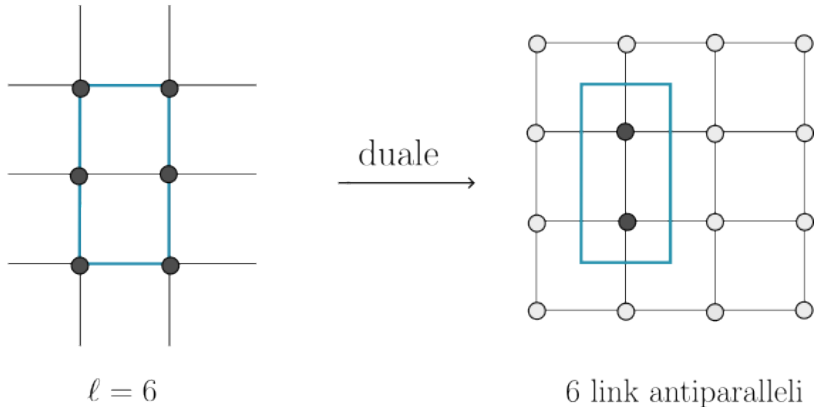
\includegraphics[width=0.53\linewidth]{Immagini/dualità KW D = 2.png}
    \caption{corrispondenza tra un poligono chiuso e il domain wall duale.}
    \label{fig: dualità KW D = 2}
\end{figure}

Inoltre, si nota che le serie in questione sono le medesime ma con diversa ragione; ci si chiede quindi se sia possibile connettere le due espressioni. Per farlo, si deve richiedere che $v = \tilde{v}$, ovvero che $e^{-2\tilde{K}} = \tanh{K}$, da cui si ricava la mappa di dualità
\begin{equation}
\label{eq: mappa di dualità}
    \tilde{K} = -\frac{1}{2}\log\tanh{K}\Longleftrightarrow \sinh{2\tilde{K}} = \frac{1}{\sinh{2K}},
\end{equation}
dove la seconda espressione mostra chiaramente come la mappa associ piccoli valori di $K$ a grandi valori di $\tilde{K}$.
\begin{obs}
    Si nota che se si applica due volte la mappa \eqref{eq: mappa di dualità} si torna al punto di partenza, infatti
    \begin{equation}
        K \longrightarrow \tilde{K} \longrightarrow \tilde{\tilde{K}} \equiv K.
    \end{equation}
\end{obs}
Avendo imposto che $v = \tilde{v}$, l'espansione ad alta temperatura \eqref{eq: funzione di partizione Ising alta T} può essere riscritta come
\begin{equation}
    Z(K) = [2\cosh^2{(K)}e^{-2\tilde{K}}]^Ne^{2\tilde{K}N}\sum_{l=0}^Lg_lv^l = [2\cosh^2{(K)}\tanh{(K)}]^N\frac{Z(\tilde{K})}{2},
\end{equation}
da cui, sfruttando le relazioni trigonometriche iperboliche, si arriva infine alla relazione di dualità di Kramers - Wannier
\begin{equation}
\label{eq: relazione Kramers-Wannier}
    Z(K) = \frac{1}{2}(\sinh{2K})^NZ(\tilde{K}).
\end{equation}
Questa relazione permette di determinare subito un'espansione se si è già calcolata la sua duale. Tuttavia, si deve notare che vale unicamente nel limite termodinamico in cui gli effetti delle condizioni al contorno sono trascurabili. Se questo non è il caso, allora bisogna tenere conto che sotto la trasformazione di dualità le condizioni al contorno per $Z(K)$ cambiano e la relazione di dualità diventa più complessa. Ad ogni modo, la relazione \eqref{eq: relazione Kramers-Wannier} implica per l'energia libera $G$ che
\begin{equation}
\label{eq: relazione Kramers-Wannier energia libera}
    \begin{split}
        G(K) &= -\frac{1}{\beta}[\log{Z(\tilde{K})} + N\log{(\sinh{2K})} - \log{2}] \\
        &= G(\tilde{K}) - \frac{N}{\beta}\log{(\sinh{2K})} + \frac{\log{2}}{\beta}.
    \end{split}
\end{equation}

\subsubsection{Temperatura critica}
La dualità di Kramers - Wannier permette di determinare in modo esatto il valore della temperatura critica $T_c$ a cui avviene la transizione ferromagnetica nel modello di Ising bidimensionale su reticolo quadrato. Siccome i termini ``aggiuntivi'' nel membro di destra della relazione di dualità \eqref{eq: relazione Kramers-Wannier energia libera} non hanno singolarità per $T > 0$, le singolarità di $G(K)$ sono mappate uno ad uno nelle singolarità di $G(\tilde{K})$, quindi $0 < K_c < K$. In generale, se ci si trova in una certa fase e se c'è una transizione di fase, ci sarà un certo punto critico $K_c$ che corrisponderà alla singolarità della funzione $G(K)$. La zona corrispondente a valori grandi di $K$, sarà quella di bassa temperatura, quindi $\tilde{K} < \tilde{K}_c < 0 $, dove valori grandi $\tilde{K}$ corrispondono a valori piccoli $K$ e viceversa. Essendoci un solo punto di singolarità ed una sola funzione $G$ si deve per forza avere
\begin{equation}
    K_c = \tilde{K}_c.
\end{equation}
Dunque, il valore critico è quello invariante per dualità. Dalla struttura del modello, dall'intuizione fisica e dall'argomento di Peierls si può assumere che vi sia un solo punto di transizione di fase: quello della transizione ferromagnetica ordine-disordine. Sotto la mappa di dualità, l'equazione \eqref{eq: mappa di dualità} implica che
\begin{equation}
    \sinh{(2K)}\sinh{(2\tilde{K})} = 1,
\end{equation}
da cui, per $K_c = \tilde{K}_c$, si trova la relazione
\begin{equation}
\label{eq: relazione per K critico}
    \begin{split}
        \sinh^2{2K_c} = 1&\quad\Longrightarrow\quad \sinh{2K_c} = \frac{e^{2K_c} - e^{-2K_c}}{2} = 1\\
        &\quad\Longrightarrow\quad e^{2K_c} = 1 + \sqrt{2}
    \end{split}
\end{equation}
che determina esattamente $K_c$ come
\begin{equation}
\label{eq: K critico}
    K_c = \frac{J}{kT_c} = \frac{1}{2}\log{(1 + \sqrt{2})} \simeq 0.44,
\end{equation}
o equivalentemente 
\begin{equation}
    kT_c = \frac{2J}{\log{(1 + \sqrt{2})}} \simeq \SI{2.27}{\joule}.
\end{equation}

\section{Soluzione di Onsager}
La prima derivazione esatta della funzione di partizione del modello di Ising bidimensionale, a campo magnetico esterno nullo è dovuta ad Onsager sfruttando il metodo della matrice di trasferimento, passando dal caso $d=1$ a quello $d=2$. Nel caso $d=1$ si aveva una catena di spin, come quella in figura \ref{fig: soluzione Onsager D = 1}, e la funzione di partizione era
\begin{equation}
    Z \propto \Tr{\TM}^N, \quad\TM\in\R^{2,2}
\end{equation}
in cui la matrice di trasferimento lega i possibili valori di $s_i$ a quelli del sito successivo $s_{i+1}$.
\begin{figure}[h]
    \centering
    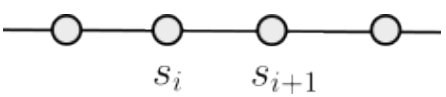
\includegraphics[width=0.35\linewidth]{Immagini/soluzione Onsager D = 1.png}
    \caption{catena di spin in $D = 1$.}
    \label{fig: soluzione Onsager D = 1}
\end{figure}

Onsager fa un discorso simile in $D = 2$. Si immagini di avere un reticolo quadrato con $N = M^2$ siti e di organizzarlo in $M$ righe e $M$ colonne, come mostrato in figura \ref{fig: soluzione Onsager D = 2}. Quindi, al posto di collegare $s_i$ ed $s_{i+1}$, la matrice di trasferimento lega i possibili valori della riga $M_i$ con i possibili valori della riga successiva $M_{i+1}$. La collezione di spin $s_A$ che descrive la configurazione di una certa riga, è una collezione del tipo
\begin{equation}
    s_A = \{ s_1^{i}, s_2^{i}, \dots, s_N^{i} \}.
\end{equation}
Data una collezione di spin che hanno valori $s_A = \pm 1$, questi oggetti corrispondono ai pesi della rappresentazione spinoriale del gruppo delle rotazioni. Questi spin possono avere $2^M$ indici, quindi la matrice $T$ è in generale una matrice di dimensione $(2^M \times 2^M)$. 
\begin{figure}[h]
    \centering
    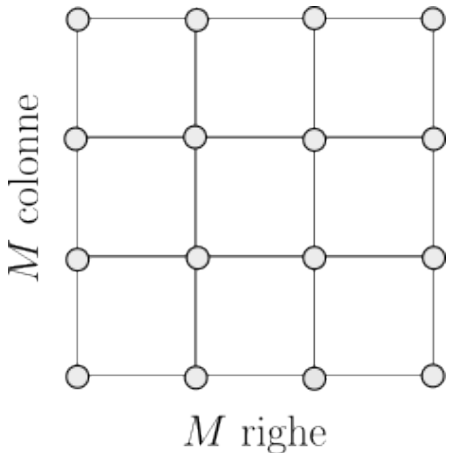
\includegraphics[width=0.3\linewidth]{Immagini/soluzione Onsager D = 2.png}
    \caption{reticolo quadrato di $N = M^2$ siti in $D = 2$.}
    \label{fig: soluzione Onsager D = 2}
\end{figure}
Quindi, già solo passando da $D = 1$ a $D = 2$ si va incontro ad una grande complicazione algebrica: lo spazio stesso della matrice tende a divergere nel limite termodinamico. Sfruttando le proprietà algebriche è possibile, anche se non è semplice, mostrare che
\begin{equation}
    Z = (2\cosh{K}e^I)^N,\quad I = \int_0^{\pi} \frac{d\phi}{2\pi} \, \log{\bigg(\frac{1 + \sqrt{1 - \kappa^2 \sin^2 \phi}}{2}\bigg)}
\end{equation}
con
\begin{equation}
    \kappa = \frac{2 \sinh(2K)}{\cosh^2(2K)} = \frac{2 \sinh(2K)}{1 + \sinh^2(2K)}.
\end{equation}
L'energia libera $G = -\log{(Z)}/\beta$ vale quindi
\begin{equation}
\label{eq: energia libera Onsager}
    G = -\frac{N}{\beta} \log(2 \cosh K) - \frac{N}{\beta} I .
\end{equation}
Per via del contributo $NI/\beta$, si ha un punto di non-analiticità legato al ``branching point'' della radice quadrata, quando
\begin{equation}
    \begin{split}
        \kappa = \kappa_c = 1 &\quad\Longleftrightarrow\quad \sinh^2(2K_c) - 2 \sinh(2K_c) + 1 = 0 \\
        &\quad\Longleftrightarrow\quad [\sinh(2K_c) - 1]^2 = 0 \\
        &\quad\Longleftrightarrow\quad \sinh(2K_c) = 1,
    \end{split}
\end{equation}
che è la stessa determinazione ottenuta dalla dualità di Kramers - Wannier nell'equazione \eqref{eq: relazione per K critico} che determina il valore critico, già trovato nella \eqref{eq: K critico}, come
\begin{equation}
    K_c = \frac{1}{2} \log(1 + \sqrt{2}) \simeq 0.44.
\end{equation}
In altre parole, $K_c$ è il punto in cui $G$ o le sue derivate possono sviluppare un comportamento singolare. In realtà, come deve essere, l'energia libera $G$ è regolare nel punto critico, infatti da $G(T,N,h = 0)$ si possono ricavare
\begin{equation}
    S = -\frac{\p G}{\p T}\bigg|_N,
    \quad
    E = -\frac{\p \log Z}{\p \beta}\bigg|_N
      = \frac{\p}{\p \beta}(\beta G)\bigg|_N.
\end{equation}
A partire dall'espressione \eqref{eq: energia libera Onsager} per $G$ si possono ricavare le espressioni esatte in termini di integrali ellittici di modulo $\kappa$, che risultano ancora continue nel punto di transizione $\kappa = \kappa_c = 1$. Quindi, per l'energia interna, per l'entropia e per l'energia libera, si trovano delle espressioni continue nel punto critico. Il fatto che ci sia questa continuità indica che se c'è una transizione di fase, questa deve essere del secondo ordine, senza calore latente. Dunque, la singolarità si deve presentare nell'espressione della capacità termica. Nel caso in cui $h = 0$, si può calcolare esattamente anche il calore specifico 
\begin{equation}
    c_N = \frac{\p E}{\p T} \bigg|_N,
\end{equation}
che risulta di nuovo espresso in termini di integrali ellittici, ma in modo tale da presentare una singolarità logaritmica per $K \to K_c$, cioè per $T \to T_c$. Si trova quindi che 
\begin{equation}
    c_N \propto kN\log{|t|},\quad t = \frac{T - T_c}{T_c}.
\end{equation}
L'andamento del calore specifico nei pressi del punto critico è logaritmico, quindi l'indice critico $\alpha$ introdotto nella \eqref{eq: legge di potenza suscettività e calore specifico} risulta essere pari a $\alpha_{\mathrm{exact}} = 0$. Infine, l'andamento del calore specifico è quello mostrato in figura \ref{fig: andamento cap. termica e M (Ising)}, in cui il calore specifico diverge avvicinandosi al punto critico.

L'espressione dell'energia libera nel caso in cui $h = 0$ non è invece sufficiente per derivare l'espressione della magnetizzazione
\begin{equation}
    M = -\frac{\p G}{\p h} \bigg|_{T,N}.
\end{equation}
Quindi, si dovrebbe accendere il campo magnetico almeno al primo ordine, fare la derivata e poi porlo uguale a zero. Risulta così ancora possibile ottenere il risultato esatto, annunciato prima da Onsager e derivato poi in dettaglio da Yang, dato da
\begin{equation}
    M(T,N,h = 0) =
    \begin{cases}
        N \bigg( 1 - \dfrac{1}{\sinh^2 2K} \bigg)^{1/8},\quad T < T_c \\[2ex]
        0,\quad T \ge T_c
    \end{cases},
\end{equation}
da cui si deduce che l'andamento della magnetizzazione ha la forma mostrata in figura \ref{fig: andamento cap. termica e M (Ising)}. Ovviamente, per la simmetria $\Z_2$ c'è anche la possibilità che si sviluppi al di sotto di $T_c$ la magnetizzazione opposta in segno. Vicino al punto critico, dalla precedente espressione segue, con $T < T_c$ (ossia per $t < 0$), che 
\begin{equation}
    M \simeq 1.22 \times N (-t)^{1/8}.
\end{equation}
Quindi, il valore esatto dell'esponente critico $\beta$ introdotto nell'equazione \eqref{eq: legge di potenza magnetizzazione}, in assenza di campo esterno, è pari a 
\begin{equation}
    \beta_{\mathrm{exact}} = \frac{1}{8}.
\end{equation}
Invece, il calcolo della suscettività magnetica è più complesso, tralasciando i dettagli matematici si trova che vicino al punto critico l'andamento della suscettività è della forma
\begin{equation}
    \chi \simeq |t|^{-7/4}.
\end{equation}
Dunque, il valore esatto dell'indice critico $\gamma$ introdotto nella \eqref{eq: legge di potenza suscettività e calore specifico} è pari a 
\begin{equation}
    \gamma_{\mathrm{exact}} = \frac{7}{4}.
\end{equation}
\begin{figure}[h]
    \centering
    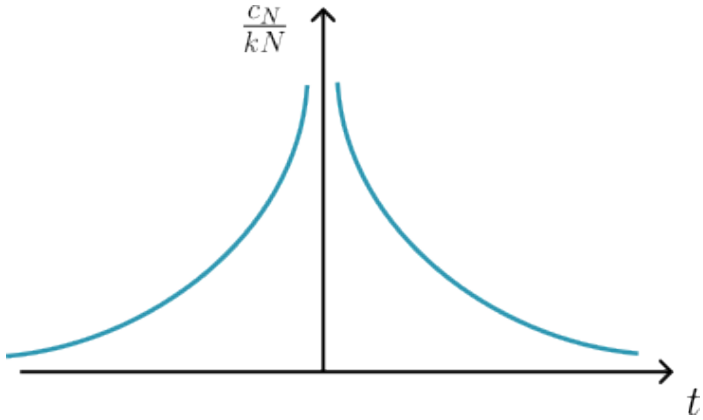
\includegraphics[width=0.4\linewidth]{Immagini/andamento cap. termica (Ising).png}
    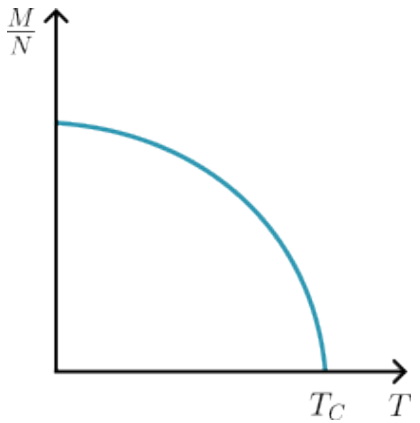
\includegraphics[width=0.3\linewidth]{Immagini/andamento M (Ising).png}
    \caption{andamento per il modello di Ising in $D = 2$ di: (i) $c_N/kN$ in funzione di $t$; $M/N$ in funzione di $T$.}
    \label{fig: andamento cap. termica e M (Ising)}
\end{figure}

\section{Correlatori}
I correlatori sono un tipo di osservabile che contengono informazioni sul modello e sul suo comportamento ai punti critici. Queste informazioni sono codificate nelle funzioni di correlazione tra spin in siti diversi e permettono di capire quanto questi si influenzino. Si consideri il correlatore
\begin{equation}
    \vmedio{s_is_j},
\end{equation}
dove $i$ e $j$ sono siti posti a distanza $r$ espressa in unità del passo reticolare. Per $r \to \infty$, i due spin non si possono influenzare e il correlatore si fattorizza secondo la ``cluster decomposition'' come
\begin{equation}
    \vmedio{s_i s_j} \underset{r \to \infty}{\longrightarrow} \vmedio{s_i}\vmedio{s_j}.
\end{equation}
Quindi, conviene introdurre il correlatore connesso $G_{ij}$ come
\begin{equation}
    G_{ij} := \vmedio{s_i - s_j}_c = \vmedio{s_is_j} - \vmedio{s_i}\vmedio{s_j}.
\end{equation}
Per un reticolo infinito o con condizioni al contorno periodiche, il valore del correlatore può solo dipendere dalla distanza relativa, per cui non dipende da dove sono posizionati i due spin. Di conseguenza, si presenta un'invarianza per traslazioni e $G_{ij}$ dipende solo dalla posizione relativa di $i$ e $j$. 

Il correlatore $G_{ij}$ si può ottenere introducendo un campo magnetico variabile da sito a sito $h_m$ in modo che
\begin{equation}
    j_m = \beta h_m
\end{equation}
giochi il ruolo di ``sorgente'' dato che si accoppia linearmente ad ogni spin, in modo analogo alla sorgente $j(x)$ che viene introdotta in Teoria dei campi. La funzione di partizione quindi è
\begin{equation}
    Z(j) = \sum_{\{s_i\}} e^{-\beta H + \sum_k j_k s_k},
\end{equation}
così che $Z(j=0)$ sia l'usuale funzione di partizione del modello di Ising a campo nullo \eqref{eq: funzione di partizione Ising D=1}. Per semplicità, si pone $j \cdot s \equiv \sum_k j_k s_k$, quindi si calcola
\begin{equation}
    \frac{\p}{\p j_n} \log Z(j)
    = \frac{1}{Z} \frac{\p}{\p j_n} \sum_{\{s_i\}} e^{-\beta H + j \cdot s}
    = \frac{1}{Z} \sum_{\{s_i\}} s_n e^{-\beta H + j \cdot s}
    \equiv \vmedio{s_n}_j,
\end{equation}
dove $\vmedio{s_n}_j$ indica il valore di aspettazione in presenza del termine di sorgente. Derivando una seconda volta si ottiene
\begin{equation}
    \begin{split}
        \frac{\p^2}{\p j_m \p j_n} \log Z(j)
        &= \frac{1}{Z} \sum_{\{s_i\}} s_m s_n e^{-\beta H + j \cdot s} - \frac{1}{Z^2}\bigg(\frac{\p}{\p j_m}Z\bigg)\sum_{\{s_i\}} s_n e^{-\beta H + j \cdot s} \\
        &= \vmedio{s_m s_n}_j - \frac{\p}{\p j_m}\log{(Z\vmedio{s_n}_i)} \\
        &= \vmedio{s_m s_n}_j - \vmedio{s_m}_j\cdot\vmedio{s_n}_j \\
        &= \vmedio{s_ms_n}_c.
    \end{split}
\end{equation}
Quindi, il correlatore connesso $G_{mn}$ nel modello di Ising a campo esterno nullo è dato da
\begin{equation}
    G_{mn} = \vmedio{s_m s_n}_c|_{j = 0} = \frac{\p^2}{\p j_m \p j_n} \log Z(j) \bigg|_{j=0},
\end{equation}
che corrisponde a dire che $\log{Z(j)}$ è la funzione generatrice dei correlatori connessi. Questa relazione si generalizza a funzioni di correlazione tra più spin, in perfetta analogia con la Teoria dei campi. Si nota anche come la derivazione precedente mostri che
\begin{equation}
    G_{mn} = \frac{\p}{\p j_m} \vmedio{s_n}_j \bigg|_{j=0},
\end{equation}
ossia il correlatore rappresenta la risposta del valore medio dello spin nel sito $n$ alla variazione del campo magnetico $h_m = j_m / \beta$ nel sito $m$. Questo perché in sostanza il fatto che ci sia una variazione di campo magnetico nel sito $m$ determina il cambiamento del valore medio in $n$ e il correlatore descrive come questo avviene.

\subsubsection{Correlatore in dimensione $D$ generica}
Si può dare un'espressione del correlatore diretto anche in termini del modello di Ising con $h = 0$ nell'espansione ad alta temperatura. In questo caso, $T > 0$ e si è nella fase disordinata in cui la simmetria non viene rotta e dove non si ha magnetizzazione spontanea, per cui $\vmedio{s_k} = 0$. Dunque, il correlatore è dato da
\begin{equation}
\label{eq: correlatore Ising D-dimensionale}
    G_{kn} = \vmedio{s_k s_n} = \sum_{\{s_i\}} s_k s_n \frac{\exp{(K\sum_{\vmedio{ij}}s_is_j)}}{Z},
\end{equation}
che nel limite ad alta temperatura, usando l'identità \eqref{eq: relazione exp(Ksisj) e cosh(K)}, diventa
\begin{equation}
    G_{kn} = \frac{1}{Z}\sum_{\{s_i\}} s_ks_n\prod_{\vmedio{ij}}[\cosh{(K)}(1 + s_is_jv)].
\end{equation}
Si vede che, con gli stessi ragionamenti fatti per derivare la funzione di partizione $Z$, che i contributi interessanti sono solo quelli corrispondenti alle possibili catene di link attivi che collegano i siti $k$ e $n$, moltiplicati per i possibili cammini chiusi. Un tipico contributo sarà della forma mostrata in figura \ref{fig: contributo correlatore D generica (alta T)}, quindi si avrà una linea che congiunge $s_k$ con $s_n$ più le possibili traiettorie chiuse, come il quadratino in alto a sinistra.
\begin{figure}[h]
    \centering
    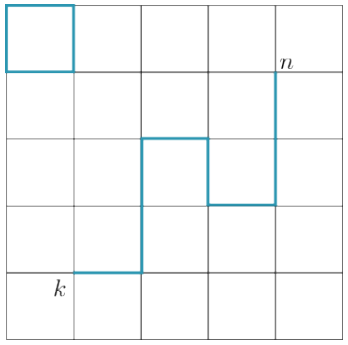
\includegraphics[width=0.3\linewidth]{Immagini/contributo correlatore D generica (alta T).png}
    \caption{contributo tipico del correlatore $G_{kn}$ nel limite di alta temperatura in $D$ generica.}
    \label{fig: contributo correlatore D generica (alta T)}
\end{figure}
I cammini chiusi, che si fattorizzano, sono gli stessi diagrammi che compaiono nella funzione di partizione. Insieme con i fattori globali $2^N(\cosh{K})^L$ si cancellano
con il fattore $Z$ a denominatore nella \eqref{eq: correlatore Ising D-dimensionale}. In definitiva il correlatore si organizza con un'espansione di potenze di $v$ data da
\begin{equation}
\label{eq: correlatore Ising D-dimensionale (espansione in serie)}
    G_{kn} = \nsum_l g_l^{(k,n)}v^l,
\end{equation}
dove il coefficiente $g_l^{(k,n)}$ è il numero di percorsi di lunghezza $l$ che congiungono i siti $k$ ed $n$. Se si ha invarianza per traslazione, tale numero dipende solo dalla posizione relativa di $k$ ed $n$, in forte analogia con il propagatore in Teoria dei campi $G(x,y) = \mybraket{\Phi(x)}{\Phi(y)}$. L'espressione \eqref{eq: correlatore Ising D-dimensionale (espansione in serie)} in traiettorie pesate da $v^l$, il quale dipende dalla lunghezza della traiettoria stessa, corrisponde alla realizzazione di $G(x,y)$ come ``path integral'' sulle traiettorie che congiungono $x$ ed $y$ pesate dal fattore $e^{-S[d]}$.

\subsubsection{Correlatore in dimensione $D = 1$}
Si studia adesso il caso 1-dimensionale. Anche qui ci si trova sempre nella fase disordinata nel limite di alta temperatura. 
\begin{figure}[h]
    \centering
    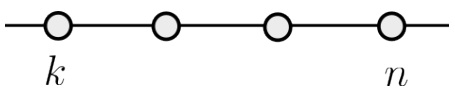
\includegraphics[width=0.3\linewidth]{Immagini/contributo correlatore D = 1 (alta T).png}
    \caption{l'unico contributo del correlatore $G_{kn}$ nel limite di alta temperatura in $D = 1$}
    \label{fig: contributo correlatore D = 1 (alta T)}
\end{figure}
In questo caso, la possibile traiettoria da $k$ ad $n$ è solamente una, mostrata in figura \ref{fig: contributo correlatore D = 1 (alta T)}, e la distanza in passo reticolare è $l = |n-k|$, quindi il correlatore è
\begin{equation}
    G_{kn} = \vmedio{s_k s_n} = \sum_{\{s_i\}} s_k s_n \frac{\exp{(K \sum_l s_l s_{l+1}})}{Z},
\end{equation}
da cui, utilizzando lo sviluppo ad alte temperature \eqref{eq: identità sviluppo alta T}, si vede come la somma sui valori di $s_i$ in qualsiasi sito richieda un numero pari di variabili $s_i$ per non annullarsi, per cui l'unico contributo non nullo è quello di una catena di link attivi dal sito $k$ al sito $n$ che fornisce
\begin{equation}
    G_{kn} = \frac{2^N \cosh^L K (\tanh K)^{|n-k|}}{2^N \cosh^L K} = (\tanh K)^{|n-k|}.
\end{equation}
Inoltre, si nota che il correlatore ha un andamento esponenziale che in particolare decresce con la distanza; quindi, si può riscrivere l'espressione del correlatore come
\begin{equation}
    G_{kn} = e^{-|n-k|/\xi},\quad \xi = \bigg(\log \frac{1}{\tanh{K}}\bigg)^{-1} > 0,
\end{equation}
dove $\xi$ rappresenta la lunghezza di correlazione e non diverge per alcuna $T > 0$.

\section{Teorema fluttuazione - risposta}
Si intende ora studiare la relazione che intercorre tra la suscettività magnetica e l'ampiezza delle fluttuazioni della magnetizzazione, dovute alla presenza di un campo esterno. Si consideri la magnetizzazione $M$ definita come nella \eqref{eq: magnetizzazione come media spin}. Se la dimensione del reticolo e/o le condizioni al contorno permettono di assumere l'invarianza per traslazioni del sistema, allora gli $s_n$ sono tutti uguali e $\vmedio{s_n}$ non dipende dallo specifico valore di $n$, che si può fissare ad esempio a $n = 1$, per cui 
\begin{equation}
    M = N \vmedio{s_1} = Nm,
\end{equation}
dove $m$ è la magnetizzazione del singolo sito. Si supponga ora di ``accendere'' un campo esterno costante $h$ (che non pregiudica l'invarianza per traslazioni essendo costante sui siti) e si calcoli la suscettività magnetica
\begin{equation}
    \chi = \frac{\p M}{\p B} = \mu_B \frac{\p M}{\p h} = N \mu_B \frac{\p \vmedio{s_1}}{\p h},
\end{equation}
dalla quale si deduce che $\vmedio{s_1}$ risponde, tramite il correlatore $G_{mn}$, alla variazione del campo esterno in ogni altro sito $n$. Per il campo costante $h$, che è uguale in tutti i siti, si ha
\begin{equation}
    h_n = \frac{j_n}{\beta} \equiv h,\quad \forall n,
\end{equation}
ossia c'è una sorgente in ognuno degli altri siti. Quindi, si vuole capire come cambia il valore di aspettazione di un qualsiasi spin, per esempio $s_1$, quando cambia il campo $h$. In sostanza, si sceglie uno spin e si va a vedere la somma dei suoi correlatori con tutti gli altri spin. Ad ogni modo, la suscettività adesso è
\begin{equation}
    \chi = N \mu_B \beta \nsum_n\frac{\p \vmedio{s_1}}{\p j_n} \bigg|_{h_n = h} = N \mu_B \beta \nsum_n G_{1n}.
\end{equation}
 Per la definizione di correlatore connesso, $G_{1n}$ è sostanzialmente diverso da zero solo se gli spin $s_1$ e $s_n$ sono correlati. Dunque, $\sum_n G_{1n} \propto \chi$ conta il numero di spin correlati con lo spin $s_1$ e, per invarianza sotto traslazioni, con qualsiasi altro spin ed è pertanto legato al range di correlazione nel sistema. Infatti, quando la suscettività $\chi$ diverge, questo segnala l'emergere di correlazione a lungo raggio nel sistema. Questo è anche legato alla divergenza della dimensione delle fluttuazioni della magnetizzazione. Infatti, valendo l'invarianza per traslazioni, $G_{kn}$ dipende solo dalla posizione relativa di $k$ e $n$, per cui
\begin{equation}
    N \nsum_n G_{1n} = \nsum_{k,n} G_{kn},
\end{equation}
ma d'altro canto si ha
\begin{equation}
    \begin{split}
        \sum_{k,n} G_{kn} = \sum_{k,n} \vmedio{s_k s_n} - \sum_{k,n} \vmedio{s_k} \vmedio{s_n} &= \bigvmedio{\left( \nsum_n s_n \right)^2} - \bigvmedio{\nsum_n s_n}^2 \\
        &= \vmedio{M^2} - \vmedio{M}^2 \\
        &\equiv\sigma_M^2.
    \end{split}
\end{equation}
Dunque, la suscettività si può scrivere come
\begin{equation}
\label{eq: relazione suscettività - magnetizzazione}
    \chi = \frac{\mu_B}{kT}\sum_{k,n}G_{kn} = \frac{\mu_B}{kT}\sigma_M^2.
\end{equation}
Questa relazione rappresenta un'istanza del teorema di fluttuazione - risposta: 
\begin{quote}
    ``la risposta del sistema ad una variazione del campo esterno $B$, codificata dalla suscettività magnetica $\chi$, è collegata all'ampiezza delle fluttuazioni della magnetizzazione espressa dalla varianza di tale quantità''.
\end{quote}
Si nota inoltre che la precedente relazione assicura che $\chi > 0$. Tuttavia, è anche da osservare come quest'ultima sia stata derivata considerando la presenza di un campo esterno $B$, così da poter effettuare la derivata e determinare $\chi$, ma resta vera se, dopo aver svolto la derivata, si pone $B = 0$. Dunque, nel caso di campo esterno nullo, le fluttuazioni della magnetizzazione spontanea  sono legate alla risposta del sistema all'accensione di un campo esterno.

\subsection{Comportamento intorno al punto critico}
La relazione fluttuazione-risposta aiuta a delineare un'immagine qualitativa del comportamento del sistema vicino al punto di transizione di fase. La suscettività magnetica diverge con un certo esponente critico $\chi \propto |t|^{-\gamma}$; ad esempio, nel modello di Ising 2-dimensionale a campo nullo, si era visto che visto che $\gamma_{\mathrm{exact}} = 7/4$. L'equazione \eqref{eq: relazione suscettività - magnetizzazione} implica allora che l'ampiezza delle fluttuazioni della magnetizzazione diverge anch'essa avvicinandosi al punto critico. Si parte ora dalla fase ordinata, per $T < T_c$, e si suppone che la magnetizzazione sia positiva, ossia $M > 0$. Le configurazioni tipiche, cioè quelle che pesano nel determinare le osservabili, sono isole di spin con spin pari $-1$ in un mare di spin pari a $+1$. La dimensione media di queste isole rappresenta la lunghezza di correlazione $\xi$ del sistema e fornisce una scala in termini della quale misurare le distanze. Andando verso il punto critico, la suscettività $\chi$ diverge e con essa diverge ad infinito la lunghezza di correlazione $\xi$. Questa divergenza è caratterizzata da un altro esponente critico del sistema con
\begin{equation}
    \xi \propto |t|^{-\nu}.
\end{equation}
Le fluttuazioni della magnetizzazione divergono, il che significa che diventano rilevanti le configurazioni con isole di tutte le dimensioni. Non c'è più una scala tipica, finita, del sistema, che appare simile a qualsiasi scala sia osservata (come un frattale). Il sistema diventa invariante per trasformazioni di scala. Siccome non vi è alcuna scala privilegiata che domina il sistema, i parametri microscopici del modello usato (il tipo di reticolo, valore di $J$, ...) non possono giocare alcun ruolo nella descrizione del sistema nelle vicinanze del punto critico. Quindi, le proprietà critiche del sistema dipendono solo da caratteristiche molto generali quali la dimensionalità $D$, il gruppo di simmetria che si rompe nella transizione, e così via. Queste sono codificate da un set di indici, o di ``esponenti'', critici $\alpha$, $\beta$ e $\gamma$ che individuano classi di universalità di sistemi, tra di loro anche molto diversi microscopicamente, accomunati dallo stesso comportamento critico. Ricapitolando, quando ci si avvicina al punto critico di transizione di fase, c'è una divergenza della lunghezza di correlazione, per cui ogni spin sente tutti gli altri e si perde la scala tipica del sistema. Questo significa che, vicino al punto critico, i dettagli non contano più, ma si vedono solo delle quantità che si comportano seguendo certe leggi di potenza e si parla di classi di universalità.

\section{Approssimazione di campo medio}
Fino ad ora non si è descritto alcun approccio che riesca a determinare il comportamento del modello di Ising per $D > 1$ in presenza di campo magnetico esterno. Un possibile, approccio è quello di tipo numerico basato sulle simulazioni di Montecarlo. Invece, un approccio analitico, basato però su forti approssimazioni, è quello del ``campo medio'', applicabile a molti modelli diversi. Per il modello di Ising, fornisce risultati tanto più corretti quanto più è alta la dimensione del reticolo, mentre per dimensioni basse questo approccio fornisce risultati solo qualitativamente validi. Anche se prevede la transizione di fase ferromagnetica, ma il set di indici critici differisce parecchio da quelli della soluzione esatta nel caso in cui $h = 0$ in $D = 2$ e da quelli forniti da accurate simulazioni numeriche. In $D = 1$ poi, anche qualitativamente si ha un disaccordo, poiché il campo medio continua a prevedere un punto di transizione del secondo ordine, mentre la soluzione esatta mostra che esso non è presente. L'approssimazione di campo medio consiste nel trascurare le fluttuazioni della magnetizzazione, o meglio nel considerarle solo all'ordine lineare. Questo è equivalente a focalizzarsi su un singolo spin $s_i$ in un qualsiasi sito $i$ e congelare tutti gli altri al loro valore medio
\begin{equation}
    \vmedio{s_k} = m = \frac{M}{N}.
\end{equation}
Pertanto, si ha una sola variabile dinamica $s_i$ che interagisce con i primi vicini, dove lo spin vale $m$. Essenzialmente, si sta dicendo che la dinamica avviene perché gli spin potrebbero cambiare, ma uno per volta. Nella pratica, si hanno solo due configurazioni che se $ h = 0$ sono come quelle mostrate in figura \ref{fig: realizzazioni ACM}, con $s_i = \pm 1$. Per queste configurazioni, il peso di Boltzmann è 
\begin{equation}
    e^{\beta J qms_i + \beta hs_i} = e^{\beta(Jqm + h)s_i},
\end{equation}
quindi la funzione di partizione è
\begin{equation}
    Z_{(i)} = \sum_{\{s_i\}}e^{\beta(Jqm + h)s_i} = 2\cosh{[\beta(Jqm + h)]}.
\end{equation}
\begin{figure}[h]
    \centering
    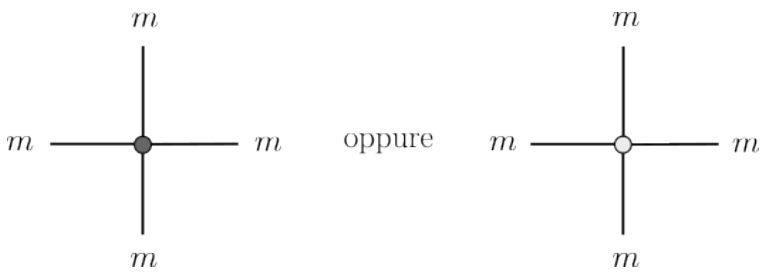
\includegraphics[width=0.6\linewidth]{Immagini/realizzazioni ACM.png}
    \caption{realizzazioni possibili nell'approssimazione di campo medio per un reticolo quadrato con $h = 0$.}
    \label{fig: realizzazioni ACM}
\end{figure}

Per consistenza, si deve anche richiedere che il valore medio di $s_i$ sia pari ad $m$, quindi
\begin{equation}
    \begin{split}
        \vmedio{s_i} = \sum_{\{s_i\}}s_i\frac{e^{\beta(Jqm + h)s_i}}{Z} &= \frac{e^{\beta(Jqm + h)} - e^{-\beta(Jqm + h)}}{Z} \\
        &= \frac{2\sinh{[\beta(Jqm + h)]}}{2\cosh{[\beta(Jqm + h)]}},
    \end{split}
\end{equation}
da cui si ricava l'``equazione di autoconsistenza''
\begin{equation}
\label{eq: equazione di atutoconsistenza}
    m = \tanh{[\beta(Jqm + h)]}.
\end{equation}
Questa è tutt'altro che un'equazione banale e non vale per qualsiasi valore di $m$, infatti è trascendente e determina i possibili valori di $m$ in funzione di $\beta$, $h$ e $J$. L'equazione \eqref{eq: equazione di atutoconsistenza} può essere risolta graficamente ponendo
\begin{equation}
    x = \beta Jqm + \beta h\quad\Longrightarrow\quad m = \frac{x - \beta h}{\beta Jq},
\end{equation}
permettendo di riscriverla come
\begin{equation}
    \frac{x - \beta h}{\beta Jq} = \tanh{x},
\end{equation}
facendo diventare il problema una ricerca grafica delle intersezioni tra le funzioni presenti ad ambo i membri, come mostrato in figura \ref{fig: soluzione grafica h = 0}. 
\begin{figure}[h]
    \centering
    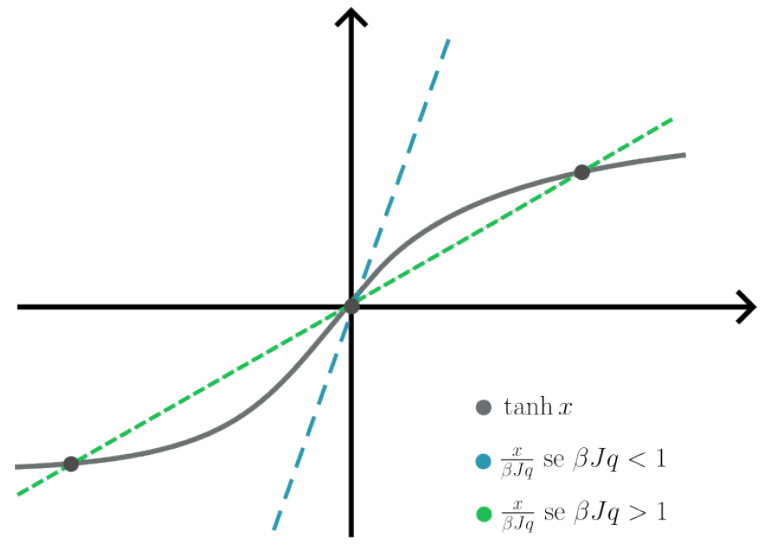
\includegraphics[width=0.5\linewidth]{Immagini/soluzione grafica h = 0.png}
    \caption{soluzione grafica per $h = 0$.}
    \label{fig: soluzione grafica h = 0}
\end{figure}
Si nota come la derivata della tangente $\tanh{x}$ sia pari ad uno nell'origine dato che
\begin{equation}
    \frac{d}{d x}(\tanh{x})\bigg|_{x=0} = \frac{1}{\coth^2{x}}\bigg|_{x=0} = 1,
\end{equation}
per cui la pendenza è di $45^\circ$. Quindi, nel caso in cui $h = 0$ si ha che:
\begin{enumerate}
    \item se $\beta J q > 1$, le due funzioni si incontrano solo in $x = 0$ ed anche $m = 0$;
    \item se $\beta J q < 1$, le due funzioni si incontrano in tre punti distinti ed $m$ può essere $m > 0$, $m < 0$ e $m = 0$.
\end{enumerate}
Pertanto, è possibile trovare delle soluzioni con magnetizzazione spontanea diversa da zero. Questo però succede soltanto quando le due fasi sono separate dal valore critico
\begin{equation}
\label{eq: K critico approssimazione campo medio}
    \beta J q = 1 \quad\Longleftrightarrow\quad K_c = \frac{1}{q} \quad\Longleftrightarrow\quad kT_c = Jq \equiv \frac{1}{\beta_c}.
\end{equation}
Questo risultato si avvicina a quello esatto o ai risultati numerici solo per $q$ alto, cioè per i reticoli regolari di dimensione alta, si raccolgono alcuni risultati in tabella \ref{tab: valori di K critico}.
\begin{table}[h]
    \centering
    \begin{tabular}{|c|c|c|}
    \hline
    $D$ & $K_c$ [campo medio] & $K_c$ [esatta o simulata] \\
    \hline
    1 & $1/2 = 0.5$   & $\infty$ \\
    \hline
    2 & $1/4 = 0.25$  & $\log(\sqrt{2}+1)/2$ \\
    \hline
    3 & $1/6 = 0.166$ & $0.221$ (MC) \\
    \hline
    4 & $1/8 = 0.125$ & $0.149$ (MC) \\
    \hline
    \end{tabular}
    \caption{valori di $K_c$ derivati dall'approssimazione di campo medio ed esatti, con (MC) si intende che la soluzione è stata trovata tramite il metodo di Monte Carlo.}
    \label{tab: valori di K critico}
\end{table}
Come si vede dalla medesima, per $D = 1$ il risultato derivante dall'approssimazione di campo medio è completamente sbagliato, poiché prevede una transizione di fase che non in realtà non c'è. Tuttavia, ci si aspetta che la soluzione si avvicini ad un risultato valido quando il reticolo è più connesso, ossia quando si hanno più primi vicini. 

D'altra parte, in presenza di $h > 0$ ci si aspetta invece che emerga una magnetizzazione, indotta dal campo esterno. In questo caso la soluzione grafica è mostrata in figura \ref{fig: soluzione grafica h > 0}. Si ha una rottura esplicita della simmetria $\Z_2$, dovuta alla presenza del termine non invariante $h\nsum_i s_i$ presente nell'hamiltoniana microscopica. Si ha poi una situazione simile, ma con il segno cambiato, se $h < 0$.
\begin{figure}[h]
    \centering
    \includegraphics[width=0.5\linewidth]{Immagini/soluzione grafica h > 0.png}
    \caption{soluzione grafica per $h > 0$.}
    \label{fig: soluzione grafica h > 0}
\end{figure}

\subsection{Equazione intorno al punto critico}
Ci si domanda se il campo medio possa prevedere anche gli indici critici nei pressi del punto critico. L'equazione di autoconsistenza \eqref{eq: equazione di atutoconsistenza} può essere scritta come
\begin{equation}
    \operatorname{arctanh}{m} = \beta Jq + \beta h = \frac{\beta}{\beta_c}m + \beta h,
\end{equation}
dove nel secondo passaggio si è usata l'equazione \eqref{eq: K critico approssimazione campo medio}. Intorno al punto critico, cioè con $\beta$ prossimo a $\beta_c$ e $h$ piccolo, si vede dalla soluzione grafica che $h$ ha una piccola magnetizzazione per ogni sito, per cui anche $m$ è piccolo. Quindi, si può sviluppare l'arcotangente iperbolica in modo da avere
\begin{equation}
    m + \frac{m^3}{3} + \cdots = m + \bigg(\frac{\beta}{\beta_c} - 1\bigg)m  + \beta h .
\end{equation}
in cui nell'ultimo termine si è trascurata la differenza perché $h$ è già piccolo. Inoltre, si ha la relazione 
\begin{equation}
    \bigg(\frac{\beta}{\beta_c} - 1\bigg) = \frac{T_c}{T} - 1  = \frac{T_c - T}{T_c} =  t \simeq \frac{T - T_c}{T_c} = -t
\end{equation}
dove è possibile confondere $T$ con $T_c$ a denominatore. Dunque, si arriva a 
\begin{equation}
    \frac{m^3}{3} \simeq  -mt + \frac{h}{Jq}.
\end{equation}
Si supponga ora di approcciare il punto critico dalla fase ordinata, cioè con $t < 0$, mantenendo $h = 0$, ossia di studiare la magnetizzazione spontanea al variare della temperatura. Quindi
\begin{equation}
\label{eq: valore di m per h = 0}
    \frac{m^3}{3} \simeq -mt\quad\Longrightarrow\quad m \simeq \sqrt{3}\,(-t)^{1/2},
\end{equation}
ovvero, in altri termini, il campo medio predice l'esponente critico
\begin{equation}
    \beta_{\mathrm{CM}} = \frac{1}{2} .
\end{equation}
Per l'approssimazione di campo medio, $\beta$ è sempre pari ad $1/2$, qualsiasi sia la dimensione. In $D = 1$ in realtà non c'è magnetizzazione spontanea, mentre in $D = 2$ il risultato esatto è $\beta_{\mathrm{exact}} = 1/8$ e in $D = 3$ i risultati numerici predicono $\beta_{\mathrm{numeric}} \sim 0.3$; pertanto, il campo medio inizia ad avvicinarsi al risultato corretto.

\subsubsection{Capacità termica}
Sempre nel caso in cui $h=0$, la predizione del campo medio per l'energia interna è
\begin{equation}
    E = \vmedio{H} = -J L m^2 = -\frac{J N q}{2} 3(-t) = \frac{3}{2} N J q \frac{T-T_c}{T_c},
\end{equation}
quando $m \neq 0$, cioè nella fase ordinata. Infine, dall'equazione \eqref{eq: K critico approssimazione campo medio} si ottiene
\begin{equation}
    E = 
    \begin{cases}
        \dfrac{3}{2} N k_B (T-T_c), \quad T < T_c,\,m\neq 0 \\[2ex]
        0, \quad T > T_c,\,m = 0
    \end{cases}
\end{equation}
dove $m = 0$ corrisponde alla fase disordinata. Dunque, la capacità termica è data da
\begin{equation}
    c_N = \frac{\p E}{\p T} =
    \begin{cases}
        \dfrac{3}{2} N k_B & T<T_c \\[2ex]
        0 & T>T_c
    \end{cases},
\end{equation}
il quale risulta evidentemente discontinuo. In particolare, per $D = 2$ la trattazione esatta prevede invece una divergenza logaritmica, con indice critico $\alpha_{\mathrm{exact}} = 0$.

\subsubsection{Suscettività magnetica}
Si supponga di accendere un campo esterno $h \ll 1$ in modo da poter calcolare la suscettività magnetica $\chi$. Nell'equazione
\begin{equation}
    \frac{m^3}{3} = -t m + \frac{h}{J q} + \cdots
\end{equation}
si può porre $m = m_0 + \epsilon$,  dove $m_0$ è la magnetizzazione spontanea che soddisfa l'equazione con $h = 0$ ed $\epsilon \ll 1$. In questo modo, si ha
\begin{equation}
\label{eq: equazione autoconsistenza punto critico}
    \begin{split}
        \frac{1}{3} ( m_0^3 + 3 m_0^2 \epsilon + 3 m_0 \epsilon^2 + \epsilon^3) &= -t(m_0 + \epsilon) + \frac{h}{Jq} \\
        m_0^2\epsilon &\simeq -t\epsilon + \frac{h}{Jq},
    \end{split}
\end{equation}
da cui, sostituendo ancora l'espressione \eqref{eq: valore di m per h = 0} per $m_0$, si trova
\begin{equation}
    -2t \epsilon = \frac{h}{J q} \quad\Longrightarrow\quad \epsilon = -\frac{h}{2Jqt}.
\end{equation}
Dunque, la suscettività magnetica è
\begin{equation}
    \chi = \frac{\p M}{\p B} = N \mu_B \frac{\p m}{\p h} = N \mu_B \frac{\p \epsilon}{\p h} = \frac{N \mu_B}{2 J q} (-t)^{-1},\quad T < T_c.
\end{equation}
Quindi, si è ottenuto un indice critico pari a $-1$. Se si ripetessero i calcoli nella fase simmetrica per $T > T_c$, si avrebbe $m_0 = 0$ e quindi $m = \epsilon \ll 1$, per cui l'equazione \eqref{eq: equazione autoconsistenza punto critico} si riduce a 
\begin{equation}
    \frac{\epsilon^3}{3} = -t \epsilon + \frac{h}{J q}
    \quad\Longrightarrow\quad \epsilon = \frac{h}{J q t},
\end{equation}
da cui si trova che la suscettività diventa
\begin{equation}
    \chi = N \mu_B \frac{\p \epsilon}{\p h} = \frac{N \mu_B}{J q} t^{-1},\quad T > T_c.
\end{equation}
Dunque, anche per la suscettività si trova una discontinuità
\begin{equation}
    \chi =
    \begin{cases}
        -\dfrac{N \mu_B}{2 J q}t^{-1},\quad T<T_c \\[2ex]
        \dfrac{N \mu_B}{J q} t^{-1},\quad T>T_c
    \end{cases}.
\end{equation}

